%loads the class that provides the titlepage and some general packages.
\documentclass{UniVieCS_Thesis} 

%add the additional packages and macros that you want to use
%here you can find some useful additional packages and macros

%Package to show algorithms
\usepackage{algorithm2e}

%package to work with glossaries
\usepackage[acronym]{glossaries}

%packages and setings to show colored code
\usepackage{listings}
\usepackage{xcolor}

\definecolor{codegreen}{rgb}{0,0.6,0}
\definecolor{codegray}{rgb}{0.5,0.5,0.5}
\definecolor{codepurple}{rgb}{0.58,0,0.82}
\definecolor{backcolour}{rgb}{0.95,0.95,0.92}

\lstdefinestyle{mystyle}{
    backgroundcolor=\color{backcolour},   
    commentstyle=\color{codegreen},
    keywordstyle=\color{magenta},
    numberstyle=\tiny\color{codegray},
    stringstyle=\color{codepurple},
    basicstyle=\ttfamily\footnotesize,
    breakatwhitespace=false,         
    breaklines=true,                 
    captionpos=b,                    
    keepspaces=true,                 
    numbers=left,                    
    numbersep=5pt,                  
    showspaces=false,                
    showstringspaces=false,
    showtabs=false,                  
    tabsize=2
}

\lstset{style=mystyle}

%package to allow comments/notes by you and other people
\usepackage[multiuser,marginclue,nomargin,inline,index]{fixme}
\definecolor{ttwgreen}{RGB}{75,135,73}
\fxusetheme{colorsig}
%\FXRegisterAuthor{tm}{atm}{\color{red}TM}
\FXRegisterAuthor{ttw}{attw}{\color{ttwgreen}TTW} % creates ttwnote, ttwwarning, ttwerror, ttwfatal commands
%\FXRegisterAuthor{mk}{amk}{\color{blue}MK}

%add your own packages or macros here
\usepackage{amssymb}

\SetKwComment{Comment}{/* }{ */}
\RestyleAlgo{ruled}

\newcommand*{\W}{\mathbf{W}}

\newcommand*{\Wlk}{\W^{(l,k)}}
\newcommand*{\Wlonekone}{\W^{(l_1,k_1)}}
\newcommand*{\Wltwoktwo}{\W^{(l_2,k_2)}}
\newcommand*{\nWlk}{n_{\Wlk}}
\newcommand*{\dWlk}{d_{\Wlk}}
\newcommand*{\nWlkXdWlk}{\nWlk \times \dWlk}
\newcommand*{\RnWlkXdWlk}{\mathbb{R}^{\nWlkXdWlk}}

\newcommand*{\vWlk}{\vX[\Wlk]}

\newcommand*{\si}{s_i}
\newcommand*{\spi}{s_{p_i}}
\newcommand*{\smi}{s_{m_i}}

\newcommand*{\sj}{s_j}
\newcommand*{\spj}{s_{p_j}}
\newcommand*{\smj}{s_{m_j}}

\newcommand*{\vXsi}[1][\theta]{\mathbf{v}_{#1}(\si)}
\newcommand*{\vXspi}[1][\theta]{\mathbf{v}_{#1}(\spi)}
\newcommand*{\vXsmi}[1][\theta]{\mathbf{v}_{#1}(\smi)}

\newcommand*{\vXsj}[1][\theta]{\mathbf{v}_{#1}(\sj)}
\newcommand*{\vXspj}[1][\theta]{\mathbf{v}_{#1}(\spj)}
\newcommand*{\vXsmj}[1][\theta]{\mathbf{v}_{#1}(\smj)}

\newcommand*{\simcos}{\operatorname{sim}_{\cos}}

\newcommand{\Indic}{\mathbf{1}}

% important update for glossaries, before document 
\loadglsentries{C) Back Matter/acronyms.tex}
\loadglsentries{C) Back Matter/glossary.tex} 
\makeglossaries %https://www.overleaf.com/learn/latex/glossaries

%shows fixme notes
\fxsetup{status=draft} % comment/delete this line if you want to your final output

\usepackage[ngerman, british]{babel} %if changed to \usepackage[ngerman]{babel} "Table of contents" changes to "Inhaltsverzeichnis", "abstract" becomes "Zusammenfassung" and "references" is translated to "Literatur".


%remove all the things you don't need and add all the things you need. you can also change the order of the elements at your will.
\begin{document}

    %Start with front matter
    
    %Choose the titlepage you want to use
    
    % --CHANGE THE TITLEPAGE HERE

% title page provided in Word by the University which can be found here 
% https://informatik.univie.ac.at/studium/hilfe-fuer-studierende/wegweiser-masterstudium/approbation-der-masterarbeit/ 
% Please pay attention to the guidelines that can be found there!
%


% There are some commands also for multiple lines. If something exceeds more than a line use the multi line commands. In the worst case adjust the vertical spaces within the class.
% -- Title Page
%\Title{Project or Select? Should gradients in post-training instance-based explanation methods be reduced in dimensionality by projecting or by selecting single components?} 
% A title exceeding one line can be created using the \TitleTwo or \TitleThree command
\TitleTwo{Select or Project? \\ Evaluating Lower-dimensional Vectors for LLM Training Data Explanations}
%\TitleThree{Select or Project? Should LLM gradients in post-training \\ instance-based explanation methods be reduced in \\ dimensionality by projecting or by selecting sub-components?}
\Who{Ing. Lukas Hinterleitner BSc} %Make sure you add all your titles! 
% A name exceeding one line can be created using the \WhoTwo command
%\WhoTwo{ FirstName \\ LastName BSc}
\Degree{Master of Science (MSc)}
\Year{2025}
\ProgrammeCode{066 645}
\ProgrammeName{Masterstudium Data Science} %Make sure it has the same Name as in the Studienblatt
\Supervisor{Univ.-Prof. Dr. -Ing. Benjamin Roth, B.Sc. M.Sc.}
%\SupervisorTwo{Second Row} % Here you can change the row under the supervisor
\CoSupervisor{0} %remove this line if there is a Co supervisor
%\CoSupervisor{Professor Co}
%\CoSupervisorTwo{Second Row} % Here you can change the row under the cosupervisor

\Titlepage %This generates the titlepage %Creates the titlepage
    
    \clearpage
	\frontmatter{}
	\thispagestyle{empty}
\chapter{Acknowledgements}

Thank you! 
\fxnote{Thank Huawei Lin for providing the illustration templates}
\clearpage
%\cleardoublepage{} %adds the aknowledgements
			%Please consider the following section of the "Formvorschriften für die gedruckte Version"
	%Im Anhang ist eine Zusammenfassung (Abstract) mitzubinden. 
	%Ist die Arbeit in einer Fremdsprache verfasst, ist im Anhang jedenfalls eine deutsche Zusammenfassung mitzubinden.
\chapter{Abstract}
		This \LaTeX{} template provides example on how to format and display text, 
		mathematical formulas, and insert tables or images. There is a lot more you 
		can do with \LaTeX{}, for more information check out https://en.wikibooks.org/wiki/LaTeX.
 % adds the abstract
	\chapter{Kurzfassung}
Das ist eine deutsche Kurzfassung meiner in Englisch verfassten Masterarbeit.
\clearpage %adds the "Kurzfassung"in german.
	\pagebreak
	
    \microtypesetup{protrusion=false}
    \tableofcontents{}
    % Use an optional list of tables / figures / algorithms / listings(code).
    \listoftables 
    \listoffigures
    \cleardoublepage{}
    \listofalgorithms
    \addcontentsline{toc}{chapter}{List of Algorithms} 
    \cleardoublepage{}
    \lstlistoflistings
    \cleardoublepage{}
    \microtypesetup{protrusion=true}
    
	\pagebreak
	
	%add your chapters here
	\mainmatter{}

    \chapter{Introduction} \label{cha:introduction}

\fxnote{As Ben said last meeting, introduce the topic in the first sentence and then explain everything in detail later.}

In recent years, machine learning applications have gained increased popularity, especially with the emergence of Large Language Models (\acrshort{llm}s) such as BERT \cite{devlin2019bertpretrainingdeepbidirectional}, GPT-3 \cite{brown2020languagemodelsfewshotlearners}, GPT-4 \cite{openai_2023}, and LLaMA-2 \cite{touvron2023llama2openfoundation}, etc. These \acrshort{llm}s employ deep neural networks (\acrshort{dnn}s), Transformers \cite{vaswani2023attentionneed}, and other components to generate coherent text based on a given textual (and occasionally visual) input. That being said, the subsequent sections will focus strictly on text-to-text language models, specifically auto-regressive language models such as GPT-1 proposed in \cite{openai_2018_generative_pre_training}.

\section{Black Boxes} \label{sec:black_boxes}
Unlike traditional machine learning models, such as Decision Trees or Linear Regression, \acrshort{dnn}s and thus \acrshort{llm}s are so-called black boxes. It is not straightforward to determine how or why such models arrive at a particular conclusion, prediction, or classification. This lack of transparency poses significant challenges in fields such as healthcare, where understanding the reason behind each decision is highly important due to the responsibility towards patients \cite{xiong2024explainableartificialintelligencexai}. Moreover, \acrshort{eu}'s \acrfull{gdpr} explicitly grants individuals the right to obtain meaningful information regarding the logic that underlies automated decisions in information systems \cite{european_commission_regulation_2016}. Explanations are therefore important not just for end users affected by these decisions but also for engineers and researchers who develop, test, and refine such systems.
\\\\
As a direct consequence, the explainability for \acrfull{ai} has become a critical research topic, gaining more and more attention under the name \acrfull{xai} \cite{https://doi.org/10.1002/widm.1391}.

\section{Explainable Artificial Intelligence} \label{sec:xai}
As noted above, the aim of \acrshort{xai} is to develop models that can be interpreted by humans, particularly for sensitive applications in fields such as military, finance and health care. Therefore, it is a key area of research for creating transparent and traceable \acrshort{ai} systems.
\\\\
Before proceeding, we must distinguish between \textbf{explainability} and \textbf{interpretability}:
\begin{itemize}
    \item \textbf{Interpretability:} Interpretability enables developers to get a better understanding of how a specific \acrshort{ai}-model works.
    \item \textbf{Explainability:} Explainability provides insight into how the system came up with a certain decision that is understandable to the end user. Explainable models provide explanations in a way that users understand why the model generated a particular conclusion.
\end{itemize}
In this article, the focus is predominantly on \textbf{explainability} rather than on \textbf{nterpretability}, although these domains frequently overlap \cite{ALI2023101805}. Since there are multiple approaches to \acrshort{xai}, a quick overview helps to categorize these approaches. According to \cite{zhao2023explainabilitylargelanguagemodels} \acrshort{llm} explainability can be structured as presented in Figure~\ref{fig:llm_explainability}.
\begin{figure}[ht]
    \centering
    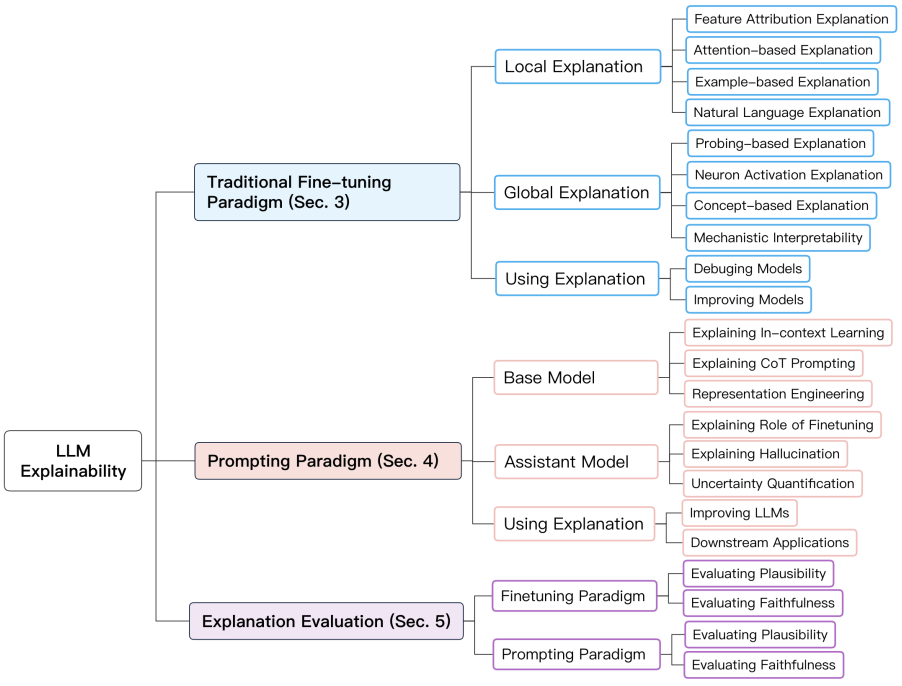
\includegraphics[width=1\textwidth]{figures/llm_explainability.png}
    \caption{Categories of LLM explainability adopted from \cite{zhao2023explainabilitylargelanguagemodels}} 
    \fxnote{Design own image}
    \label{fig:llm_explainability}
\end{figure}
The focus in the article is on the \textit{traditional fine-tuning paradigm}, more on that later. In this context, the key distinction between \textit{local explanation} and \textit{global explanation} is that the former aims to clarify individual model predictions, while the latter seeks to shed light on the internal workings of language models.
\\\\
The method introduced in the upcoming chapters falls under the \textit{local explanation} category and specifically under \textit{example-based explanation}, as it targets individual instances rather than isolated features \cite{zhao2023explainabilitylargelanguagemodels}.

\section{Problem Statement} \label{sec:problem_statement}
As mentioned above, this work focuses on example-based (instance-based) explanations. More specifically, the objective is to determine how effectively a model can identify the original data point given a paraphrased version of it. To that end, each sample in a supervised fine-tuning dataset is paraphrased and stored alongside its original counterpart. This paraphrasing is performed using an external model (GPT-4o mini \cite{openai_2024_gpt4o_mini}) or the model under evaluation. The original and paraphrased samples are then passed through the model, and the respective gradients for both samples are calculated. The cosine similarity is then employed to measure the degree to which these gradients align, providing a score between -1 and 1. The cosine similarity captures the cosine of the angle between two non-zero vectors, yielding a measure of similarity between the gradients. By comparing all gradients, we obtain a ranking and a corresponding score that indicate how well gradient-based explanations detect the original sample when given a paraphrased version for a given model.
\\\\
By using this method, the evaluation of these gradient-based explanations will not require a retraining of the model since it only computes how the model's output changes with respect to small changes in the input by paraphrasing. In simple terms, the original and paraphrased inputs are piped through the model and the difference of the respective gradients is measured. Hence, no additional training loop or parameter tuning is required. 
\\\\
While instance-based explanations are well known in the context of classification models, they have been relatively unexplored for \acrlong{llm}s. Given that \acrlong{llm}s can contain many parameters (for example, LLaMA 3.1 has up to 405 billion parameters \cite{meta_ai_llama_3_1}), the associated computations can be very expensive. Specifically, the proposed approach calculates at least one gradient for each layer per training sample. Consequently, for a single sample, the combined gradients can be as large as the entire model. In the case of LLaMA 3.1 (405B), the gradients of a single example contain up to 405 billion floating-point values.
\\\\
However, the proposed methodology contributes both a mechanism and a dataset to evaluate and benchmark instance-based explainability techniques. In addition, other explanation methods can be substituted for the gradient-based approach described here. Moreover, as already stated, this type of benchmark does not require retraining of the model, which makes it particularly well suited for already fine-tuned \acrshort{llm}s.

\subsection{Layer Importance}
Because \acrshort{llm}s incorporate numerous components, such as embedding, Transformer decoder, and \acrshort{mlp} layers \cite{Rosenblatt1958-mn}, it is beneficial to assess which layers have the greatest influence compared to all gradients of the layers. Here, we investigate how each layer influences both the ranking and the overall score of the attributions associated with the paraphrased samples.
\\\\
As already stated above, gradients of \acrshort{llm}s can be high-dimensional and hence expensive to work with. 

\fxnote[inline]{Further elaborate on layer selection, dimensionality reduction, other papers are just randomly picking layers (MLP)}

\fxnote[inline]{Size of gradients, random projections, layer importance, benefits of greedy selection etc. }

    \chapter{Related Work}
According to \cite{zhao2023explainabilitylargelanguagemodels}, the training of \acrshort{llm}s can be categorized into two paradigms, namely \textit{traditional fine-tuning} and \textit{prompting} depending on how they are adapted for downstream tasks (see Figure~\ref{fig:llm_explainability}). 
\\\\
In \textit{traditional fine-tuning}, the \acrlong{llm} is pre-trained on a large corpus of unlabeled text data and further fine-tuned on labeled data tailored to a specific domain and bench-marked accordingly (for example, the GLUE benchmark \cite{wang2019gluemultitaskbenchmarkanalysis}). In the \textit{prompting} paradigm the so-called \textit{prompts} enable the model to behave in a certain way without retraining it, enabling zero-shot, one-shot and few-shot learning without requiring additional training data \cite{brown2020languagemodelsfewshotlearners}. 
\\\\
As stated in section~\ref{sec:xai} and shown in Figure~\ref{fig:llm_explainability}, \textit{Gradient-Based Explanation} is a subcategory of \textit{feature attribution-based explanation}. However, the approach presented in this article falls under \textit{example-based explanation} (or in other words \textit{instance-based explanation}) but also uses a kind of gradient-based solution and therefore \textit{gradient-based explanation} will be briefly described in the next section.

\section{Gradient-Based Explanation}
The importance of each input feature can be evaluated using gradient-based attribution techniques. This is achieved by analyzing the partial derivatives of the output with respect to each input dimension. The magnitude of the derivatives reveals how sensitive the output is to changes in the input. This method can generally be formulated as $s_j=\frac{\partial f(x)}{\partial x_j}$, where $f(x)$ is the function of the neural network and $x_j$ is the input vector \cite{zhao2023explainabilitylargelanguagemodels}. 
\\\\
However, the approach covered in this article will use the full gradients of each model layer with respect to a single training example instead of a single feature dimension; hence, it is more important to shed more light on example-based explanations and, therefore, different example-based variants will be briefly discussed in more detail below. Not all of them are actually completely related to the proposed approach in this article; however, it still makes sense to establish an outline of the closely and not so closely related topics to gain an overview before jumping into details of the proposed approach.
\\\\
Nevertheless, not all gradient-based explanation methods are tied to different feature dimensions, and gradients can also be useful in the context of example-based explanation. More about that is outlined in Section~\ref{subsec:data_influence}.

\section{Example-Based Explanation}
Example-based explanations offer a way to explain a model's behavior based on individual examples (or instances) \cite{koh2020understandingblackboxpredictionsinfluence}. In other words, they offer a way to identify how a model's output changes on the basis of different inputs. Furthermore, according to \cite{zhao2023explainabilitylargelanguagemodels}, example-based explanations can be divided into three categories: \textit{adversarial examples}, \textit{counterfactual explanations}, and \textit{data influence}. 

\subsection{Adversarial Example}
\acrlong{lm}s have been shown to be vulnerable to small adjustments in their input data. Although these carefully constructed changes may not be noticeable to humans, they can influence the output of a model. In the beginning, adversarial examples were based on word-level alterations such as small errors, removal, and insertion. Over time, more advanced token-level perturbation methods such as \textit{TextFooler} \cite{jin2020bertreallyrobuststrong} were published. These approaches specify important words on embedding similarity, same part of speech, etc. and are correspondingly modified. However, methods relying on word embeddings are limited in sentence representation compared to contextualized representations, which often lead to incoherent pieces.
\cite{wang2022semattacknaturaltextualattacks} proposed \textit{SemAttack}, a framework that can be used for different embedding spaces, such as type space, knowledge space, and contextualized semantic space. Once the input tokens are transformed to an embedding space, the perturbed embeddings are optimized iteratively until a specific goal is met. One of the experiments shows that by replacing 5\% of the words, the accuracy of BERT drops from 70.6\% to 2.4\%. 
\\\\
\fxnote{Describe counterfactual explanation here! Some counterfactual methods also use paraphrasing.}
%\subsection{Counterfactual Explanation}
%asdf

\subsection{Data Influence} \label{subsec:data_influence}
The notion of \textit{data influence} originally came from statistics. There, the influence of a particular data point on a model's parameters was measured by simply removing it during training. Regarding data influence methods, there are two important distinctions based on when gradients are obtained:
\subsubsection{Static, Gradient-Based Influence Estimation}
This type of explanation method got its name because it measures the influence only on the final model parameters $\theta^{(T)}$, which are static after training is finished. Compared to dynamic methods (see \nameref{subsubsec:dynamic_gradient_based_influence_estimation} below), the static estimator is computationally more efficient since it only relies on the final model parameters. However, it has less information to estimate and therefore provides limited insight. The approach proposed in this article also falls into this category, as it depends on an already trained or fine-tuned model and calculates gradients with respect to single input examples \cite{Hammoudeh_2024}.
\\\\
Using influence functions, a static data influence estimator, the authors of \cite{koh2020understandingblackboxpredictionsinfluence} are able to explain the predictions of a black-box model by tracing back to the specific training examples that contributed the most to each prediction. To make this setting suitable for large-scale deep learning models, their approach relies on approximating these influence functions by using only gradient and Hessian-vector products. 
\\\\
The contributors of \cite{guo2021fastifscalableinfluencefunctions} demonstrate an improved application of influence functions for model debugging by using \acrfull{knn} to narrow down the search space to a subset of good candidate data points. However, computing a high-dimensional inverse Hessian-vector product is very expensive and, therefore, influence functions are difficult to scale to \acrlong{llm}s. 
\\\\
Consequently, in 2023, Anthropic scaled the idea of influence functions for \acrshort{llm}s with up to 52 billion parameters by an \acrfull{ekfac} approximation. In the article, they use influence functions to examine generalization patterns of \acrlong{llm}s. According to the authors, influences approach near zero when the order of the key phrases in a prompt is changed \cite{grosse2023studyinglargelanguagemodel}. 

\subsubsection{Dynamic, Gradient-Based Influence Estimation} \label{subsubsec:dynamic_gradient_based_influence_estimation}
Dynamic gradient-based estimators approach the analysis by reconstructing the training's data influence based on the model parameters during training, e.g. $\theta_0,...,\theta_T$. In the case of \acrlong{llm}s, working with the model parameters for each training checkpoint is more computationally expensive. However, they can be more precise than static estimators because they can harness more underlying information about the changes in the model with respect to the training data \cite{Hammoudeh_2024}.
\\\\
Various data influence methods are discussed in the previous sections. Additional categories and more details go beyond the scope of this chapter. Hence, Figure~\ref{fig:influence_analysis_methods} illustrates the categorization of the seven primary point-wise influence analysis methods with examples of specific algorithms.
\begin{figure}[ht]
    \centering
    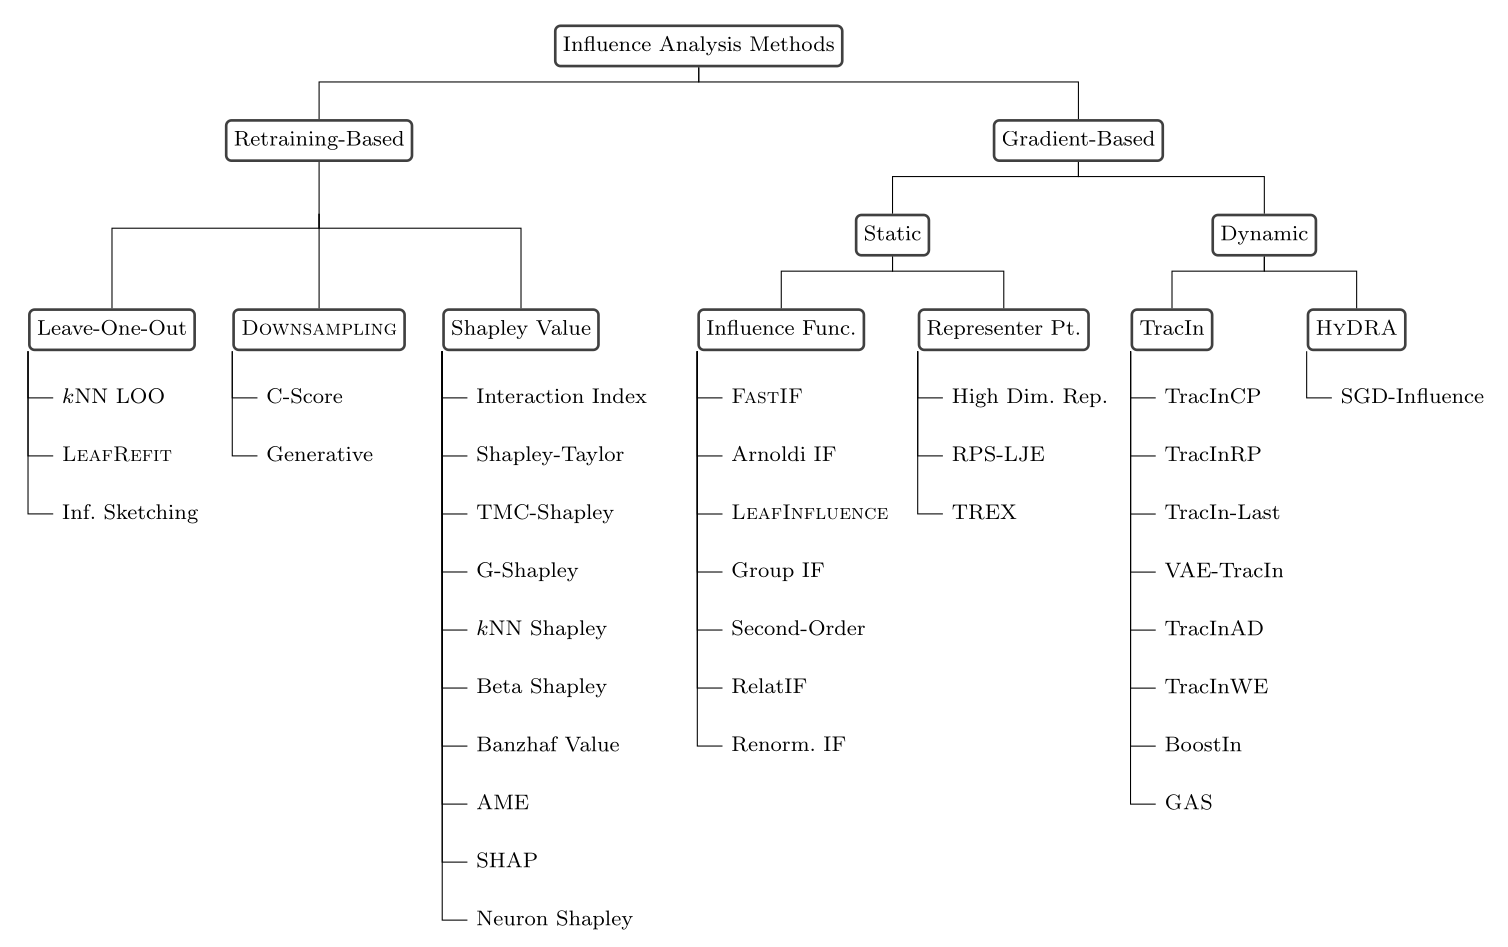
\includegraphics[width=1\textwidth]{figures/influence_analysis_methods.png}
    \caption{Categorization of different influence analysis methods and corresponding algorithms adopted from \cite{wang2024datashapleytrainingrun}}
    \fxnote{Design own image to match thesis style}
    \label{fig:influence_analysis_methods}
\end{figure}

\section{Paraphrased Corpora Analysis}
The authors of \cite{wang2024datashapleytrainingrun} did an experiment that is similar to the approach proposed in this article. There, the robustness of In-Run Data Shapley and influence functions is evaluated by identifying relevant individual corpora that have been paraphrased. They also calculate a rank based on the original training corpus and its paraphrased versions. For comparison, the BM25 \cite{bm25} distance is used as an oracle to assess the lexical similarity between the paraphrased versions and the original corpora, rather than the semantic similarity. Even with completely rewritten corpora, the corresponding original samples still rank very high according to In-Run Data Shapley and influence functions compared to BM25.
\\\\
\fxnote{Additional notes on related work (to be removed):}
\\\\
\fxnote{Further look into the paraphrased corpora analysis above to identify differences and similarities and elaborate an them.}
\\\\
\fxnote{Find related papers regarding layer selection/importance/influence with respect to predictions or explanations.}
\\\\
\fxnote{Also mention the pros of example based explanations: model-invariant as long as the model architecture uses gradients of a loss function based on inputs and outputs with respect to the input. Also, mention that the combination of gradient and example-based explanations does not require a retraining of the model.}
\\\\
\fxnote{Maybe write also about papers regarding LLMs (Attention, Transformer, ARLM vs. MLM), OLMo, Open-Instruct, Lima Dataset as well, since they are the basis of the experiments, etc.}
%\\\\
%\fxnote{Eventually include forward-, backward-pass, optimizers, etc.}

\section{Dimensionality and Performance}

\subsection{Traditional Dimensionality Reduction Techniques}
random projection

\subsection{Layer Selection}
\fxnote{introduce transformer architecture to establish connection to individual layers and gradient}

\subsubsection{Cornerstone Layers}
\cite{yeh2022betterlanguagedatainfluence}
    \chapter{Gradient Similarity as a Method for Explanation}\label{cha:gradient_similarity}

\section{Instance-based Explainability Methods}
\fxnote{Establish setting of instance-based and furthermore gradient-based explanations, etc.}

\section{Fine-Tuning Setting}\label{sec:fine_tuning_setting}
Given a fine-tuning training dataset $D = \{s_i\}_{i=0}^N$, where $s_i$ is the $i$-th sample that contains a sequence of tokens. In the scope of this article, the term \emph{original} refers to samples in this dataset. Each of these samples contains instructions and generations, where $s_i^{-P_i},...,s_i^{-1}$ denote the tokens of the $i$-th instruction prompt of length $P_i$, and $s_i^0,...,s_i^{G_i}$ denote the tokens of the $i$-th generation for the $i$-th prompt with a length of $G_i$.
\\\\
Then the training of an \acrshort{llm} can be formulated as follows: 
\begin{equation}
    \hat{\theta} = \arg\min_{\theta} \frac{1}{\sum_{i=0}^{N} G_i} \sum_{i=0}^{N} \sum_{j=0}^{G_i} \mathcal{L}(s_i^j, \theta)
    \label{eq:llm_loss_function}
\end{equation}
where $\theta$ represents the parameters of the model and $\mathcal{L}(\cdot, \theta)$ is the loss function. The term $\frac{1}{\sum_{i=0}^{N} G_i}$ in equation \ref{eq:llm_loss_function} is the total number of generation tokens in the entire training set. Usually, for the \acrshort{llm} objective, the loss is $\mathcal{L}(s_i^j, \theta) = -\log p_\theta(s_i^j \mid s_i^{-P_i}, \ldots, s_i^{j-1})$ the negative log-likelihood of the correct token given all previous tokens. \fxnote{Maybe explain where the probabilities are coming from --> softmax} Modern \acrshort{llm} architectures use adapted versions of it or may use other loss functions. However, in this setting, the choice of loss function does not matter as long as it suits language modeling. Let $\mathcal{L}(s_i, \theta) = \frac{1}{G_i} \sum_{j=0}^{G_i} \mathcal{L}(s_i^j, \theta)$, be the loss per sample which will be relevant in the following sections.
\\\\
Usually, machine learning models are trained using batches of training data. In the setting of this article, the batch size is set to exactly one to measure phenomena for single instances. Hence, in the training process, for iteration $a$, the parameters are updated from $\theta_{a-1}$ to $\theta_{a}$ depending only on the training sample $s_a$. 
\\\\
Modern \acrshort{llm} training still relies on the original idea of gradient descent to update the model weights despite being more advanced in terms of convergence, regularization, memory-efficiency, etc., for example, LAMB \cite{you2020largebatchoptimizationdeep}. However, in the proposed setting, we are only looking at the gradients of the loss function with respect to each individual training sample without updating the model weights correspondingly; therefore, establishing the idea of gradient descent is sufficient here. The formulation of gradient descent for this setting is shown in equation \ref{eq:gradient_descent}:
\begin{equation}
    \theta_{a+1} = \theta_a - \eta_a \nabla_{\theta} \mathcal{L}(s_a, \theta_a)
    \label{eq:gradient_descent}
\end{equation}
where $\eta_a$ is the learning rate in iteration $a$ and $\nabla_{\theta} \mathcal{L}(s_a, \theta_a)$ denotes the gradient of the loss function given $s_a$ and the current model parameters $\theta_a$ with respect to $\theta$. \cite{lin2024tokenwiseinfluentialtrainingdata}. In other words, the gradients determine how the model weights are updated based on the given training data. Hence, the gradient $\nabla_{\theta} \mathcal{L}(s_a, \theta_a)$ contains information on how the model parameters $\theta$ will be updated depending on the training data sample $s_a$. With this in mind, the effect of the gradient based on single samples will be analyzed in detail in the following chapters.
\fxnote{should I cite gradient descent, etc.?}

\section{Paraphrasing a Dataset}\label{sec:paraphrasing_a_dataset}
The idea is to take a dataset $D$ on which a model was fine-tuned and paraphrase it using another \acrshort{llm}. When paraphrasing, we obtain $D_p = \{s_{p_i}\}_{i=0}^N$, a dataset where the inputs and the outputs, in other words, the prompt and the generation, are paraphrased. Hence, the semantics of the samples are preserved, while the syntax and word choice differ between $D$ and $D_p$. For that, the prompt and the generation for each sample $s_i$ are individually paraphrased to retrieve a new sample $s_{p_i}$, as illustrated in Equation \ref{eq:paraphrasing}. As a reminder, each sample is basically a tuple containing an instruction and a generation. For simplicity, let us introduce $s_{i_P}$ and $s_{i_G}$ which represent the prompt and the generation of the $i$-th sample, respectively, such as $s_i = (s_{i_P}, s_{i_G}) = (s_i^{-P_i},...,s_i^{-1}, s_i^0,...,s_i^{G_i})$.
\begin{equation}
    s_{p_i} = 
    (
    s_{p_{i_P}},
    s_{p_{i_G}}
    ) =
    (
        s_{p_i}^{-P_i},...,s_{p_i}^{-1},
        s_i^0,...,s_{p_i}^{G_i}
    ) = 
    (
        \operatorname{LLM_{para}}(s_{i_P}), 
        \operatorname{LLM_{para}}(s_{i_G})
    )
    \label{eq:paraphrasing}
\end{equation}
As mentioned above, $s_{p_i}$ denotes the paraphrased version of the $i$-th sample representing a tuple of the paraphrased prompt $s_{p_{i_P}}$ and the paraphrased generation $s_{p_{i_G}}$. The function $LLM_{para}$ in Equation \ref{eq:paraphrasing} basically represents an \acrshort{llm} that is used to paraphrase a sequence of tokens as mentioned above and will be further illustrated in Section \ref{sec:paraphrasing_samples}.
\\\\
Furthermore, another paraphrasing setting is established by using the model under evaluation to generate the output with the paraphrased instruction prompt $s_{p_{i_P}}$ as input. This basically generates another dataset $D_m = \{s_{m_i}\}_{i=0}^N$ that is used for further evaluation in this context. As the other samples of the datasets $D$ and $D_p$, each sample $s_{m_i}$ of $D_m$ represents a tuple of prompt $s_{m_{i_P}}$ and generation $s_{m_{i_G}}$, as shown in Equation \ref{eq:model_generated_sample}.
\begin{equation}
    s_{m_i} = 
    (
    s_{m_{i_P}},
    s_{m_{i_G}}
    ) =
    (
        s_{p_i}^{-P_i},...,s_{p_i}^{-1},
        s_{m_i}^0,...,s_{m_i}^{G_i}
    ) = 
    (
        s_{p_{i_P}}, 
        \operatorname{LLM}(s_{p_{i_P}})
    )
    \label{eq:model_generated_sample}
\end{equation}
Technically, $s_{m_{i_G}} = s_{p_{i_G}}$, but for clarity $s_{m_{i_G}}$ will be denoted independently to establish its affiliation to $D_m$ and not be confused with an instruction for a sample in $D_p$. The function $LLM(\cdot)$ in Equation \ref{eq:model_generated_sample} basically returns the generation of the current \acrshort{llm} under evaluation and takes in a sequence of tokens $s_i^{-P_i},...,s_i^{-1}$. The dataset $D_m$ is generated to add an additional layer of obfuscation when considering the original $D$ and the paraphrased one $D_p$.
\\\\
Given that, the following two settings are established and, for simplicity, will be named accordingly in the following article:
\begin{itemize}
    \item \textbf{Paraphrased}: This setting refers to the evaluations regarding the dataset $D_p$. Samples $\spi$ in this setting will be called paraphrased samples.
    \item \textbf{Model-Generated}: This setting refers to the evaluation regarding the dataset $D_m$. Alternatively, in this setting, the samples $\smi$ will be called model-generated samples.
\end{itemize}

\section{Language Model Components}
Modern \acrlong{llm}s still rely on the Transformer architecture to create appropriate text based on an input prompt. In other words, autoregressive language models, for example, the \acrfull{gpt} model series from OpenAI, predict tokens based on a sequence of input tokens using an adapted decoder-only architecture inspired by the original Transformer \cite{vaswani2023attentionneed}.

\subsection{Different Layers and Components}\label{ssec:different_layers_and_components}
Hence, we have many trainable parameters from different components. Some of them, for example, activation functions, input layer normalization, post-attention layer normalization, etc., usually included in every \acrlong{llm}, are not trainable and therefore no gradient of the loss function with respect to these components is calculated. For a generic \acrshort{llm} that takes in a sequence of tokens, we might have the following trainable parameters without considering positional encoding, etc.:
\begin{itemize}
    \item \textbf{Input Embedding}: This parameter takes in an already tokenized and encoded sequence and transforms it into the embedding space using, for example, a matrix $\mathbf{E} \in \mathbb{R}^{|V| \times d_x}$. 
    
    \item \textbf{Multiple Transformer Block}:
    Each transformer block is applied multiple times depending on the model architecture. A generic transformer decoder consists of:
    \begin{itemize}
        \item \textbf{Self-Attention}: Three matrices representing the query, key, and value weights in self-attention:
            \begin{align*}
                  \mathbf{W}^{(q)} \in \mathbb{R}^{d_x \times d_q},  
                  \mathbf{W}^{(k)} \in \mathbb{R}^{d_x \times d_k},  
                  \mathbf{W}^{(v)} \in \mathbb{R}^{d_x \times d_v}.
            \end{align*}\cite{dl4nlp}
        \item \textbf{Multiple MLP Projections}: Each transformer block also contains a position-wise feed-forward network (in this example, a two-layer MLP). For every block, the model learns
            \begin{align*}
              \mathbf{W}^{(1)} &\in \mathbb{R}^{d_x \times d_{ff}}, & \mathbf{b}^{(1)} &\in \mathbb{R}^{d_{ff}},\\
              \mathbf{W}^{(2)} &\in \mathbb{R}^{d_{ff} \times d_x}, & \mathbf{b}^{(2)} &\in \mathbb{R}^{d_x},
            \end{align*}
              where $d_{ff}$ is the hidden width of the MLP. It can be written as one liner: $\text{MLP}(x)=\mathbf{W}^{(2)}\bigl(\text{ReLU}(\mathbf{W}^{(1)}x+\mathbf{b}^{(1)})\bigr)+\mathbf{b}^{(2)}$, where $x$ is a training sample or in the case of \acrlong{llm}s, the output of a previous layer component.
    \end{itemize}
    
    \item \textbf{Output Embedding}: A final linear layer projects the network output back to vocabulary logits. In some \acrshort{llm}s, the weights are tied to the input embedding \cite{press2017usingoutputembeddingimprove}:
          \begin{align*}
              \mathbf{W}^{(o)}=\mathbf{E}^{\top}\in\mathbb{R}^{d_x \times |V|}
          \end{align*}
          where $|V|$ is the size of the vocabulary. (Some models keep an independent $\mathbf{W}^{(o)}$ instead.)
\end{itemize}
As already mentioned, this is just a simplified illustration of the trainable parameters an \acrshort{llm} could have. In practice, the attention mechanism can be divided into multiple attention heads to capture different semantics in each head. For a detailed illustration of the Transformer decoder, see the original paper "Attention Is All You Need"~\cite{vaswani2023attentionneed}. Now that the notion of some trainable parameters for \acrlong{llm}s is put into context, the original assumption of gradient similarity is established in the following sections.

\section{Gradient Similarity between Samples}
TODO: illustrate the general idea; use general notation of similarity between gradients of different samples.

\fxnote{the upcoming section only covers equation with $\spi$. make clear, that the calculation also are valid for $\smi$}

\subsection{Gradient Flattening}\label{subsec:gradient_flattening}
Equation~\ref{eq:gradient_descent} illustrates how gradient descent updates the model parameters for training iteration $a$ and the current model parameters $\theta_a$. However, the setting in this article focuses on already fine-tuned models, and hence only the final model parameters $\theta_T$ are used for gradient computations. For example, the loss function gradient for a sample $s_i$ and the trained model parameters $\theta_T$ w.r.t. the model parameters $\theta$ is denoted as $\nabla_{\theta} \mathcal{L}(s_i, \theta_T)$.
\\\\
As illustrated in Subsection~\ref{ssec:different_layers_and_components}, the model parameter space $\theta$ consists of many different variations of matrices with different sizes and dimensions. For simplicity, denote the parameter space $\theta$ as a generic set of parameter matrices
$\{\Wlk\}_{l=0}^L$, where $\Wlk \in \RnWlkXdWlk$. Here, $L$ denotes the number of layers, and $k$ just the $k$-th weight in layer $l$, where $k \in 0,\dots,K_l$ and $K_l$ is the number of weights inside layer $l$. Depending on which \acrshort{llm} is used, the number of layers $L$, the weights inside these layers, and the dimensions of those weights $\RnWlkXdWlk$ differ in size and dimension. The size of the model, in other words, the number of trainable parameters a model has, is shown in Equation \ref{eq:number_model_parameters}.
\begin{equation}
    M = \sum_{l=0}^{L} \sum_{k=0}^{K_l} \nWlk + \dWlk
    \label{eq:number_model_parameters}
\end{equation}
As an example, today, there are many different \acrlong{llm}s with different sizes, for example, Llama 3.1 consists of 405 billion parameters \cite{grattafiori2024llama3herdmodels} and, hence, for Llama 3.1, $M \approx 405,000,000,000$.
\\\\
For simplicity, call $\nabla_{\theta} \mathcal{L}(s_i, \theta_T)$ the full model gradient for sample $s_i$. To compute this full model gradient, the gradients w.r.t. to each model weight $\nabla_{\mathbf{W}^{(l,k)}} \mathcal{L}(s_i, \theta_T) \in \RnWlkXdWlk$ have to be calculated and combined to represent the gradient w.r.t. the whole parameter space. After the computation of each individual weight gradient $\nabla_{\Wlk} \mathcal{L}(s_i, \theta_T)$, they are flattened into a gradient vector that can be calculated as: 
\begin{align*}
    \mathbf{v}_{\Wlk}(s_i)
    \;:=\;
    \operatorname{vec}_r\bigl(\nabla_{\Wlk}\mathcal L(s_i,\theta_T)\bigr)
    \;\in\;\mathbb R^{\,\nWlk\dWlk}.
\end{align*}
The row-major vectorization function $\operatorname{vec}_r(\cdot)$, is the mapping $\operatorname{vec}_r:\mathbb{R}^{m \times n} \to \mathbb{R}^{mn}, \quad \mathbf{a} = \operatorname{vec_r}(\mathbf{A})$, where $\mathbf{A} = [A_{ij}] \in \mathbb{R}^{m \times n}, \quad i = 0, \ldots, m-1, \quad j = 0, \ldots, n-1$. Then this row-major vectorization is explicitly written as follows:
\begin{align*}
    \mathbf{a} = \operatorname{vec}_r(\mathbf A)=
    \begin{bmatrix}
    A_{0,0}\\ A_{0,1}\\ \cdots\\ A_{0,n-1}\\
    A_{1,0}\\ A_{1,1}\\ \cdots\\ A_{1,n-1}\\
    \vdots\\
    A_{m-1,0}\\ \cdots\\ A_{m-1,n-1}
    \end{bmatrix}
    \;\in\;\mathbb{R}^{mn}.
\end{align*}
\cite{curtarelli2023generalizedvectorizationinverse}. For example,
\begin{align*}
    \mathbf A=
    \begin{bmatrix}
    1 & 2 & 3\\
    4 & 5 & 6
    \end{bmatrix} \;\in\; \mathbb{R}^{2\times3}, 
    \quad 
    \operatorname{vec}_r(\mathbf A)=
    \begin{bmatrix}
    1\\2\\3\\4\\5\\6
    \end{bmatrix}.
\end{align*}
To combine all vectorized layer gradients $\mathbf{v}_{\Wlk}(s_i)$ for sample $s_i$, define the collector operator $\operatorname{col(\cdot)}$ as follows:
\begin{align*}
    \operatorname{col}(x_1,\dots,x_m) \;:=\;
    \begin{bmatrix}
    x_1 \\ \vdots \\ x_m
    \end{bmatrix} \; \in \; \mathbb{R}^{\sum_{j}{d_j}}, \quad \text{where} \; x_j \in \mathbb{R}^{d_j}.
\end{align*}
With the above properties and operators in mind, the full flattened gradient vector for sample $s_i$ is defined as 
\begin{align*}
    \vXsi[\theta]
\;:=\;
\operatorname{col}\bigl( \vXsi[\W^{(0,0)}], \vXsi[\W^{(0,1)}], \dots, \vXsi[\W^{(L,K_L)}] \bigr)
\; 
\in\; \mathbb{R}^{M}.
\end{align*}
For better understanding, the whole gradient flattening process covered in this subsection is illustrated in Figure \ref{fig:gradient_flattening}.
\begin{figure}[ht]
    \centering
    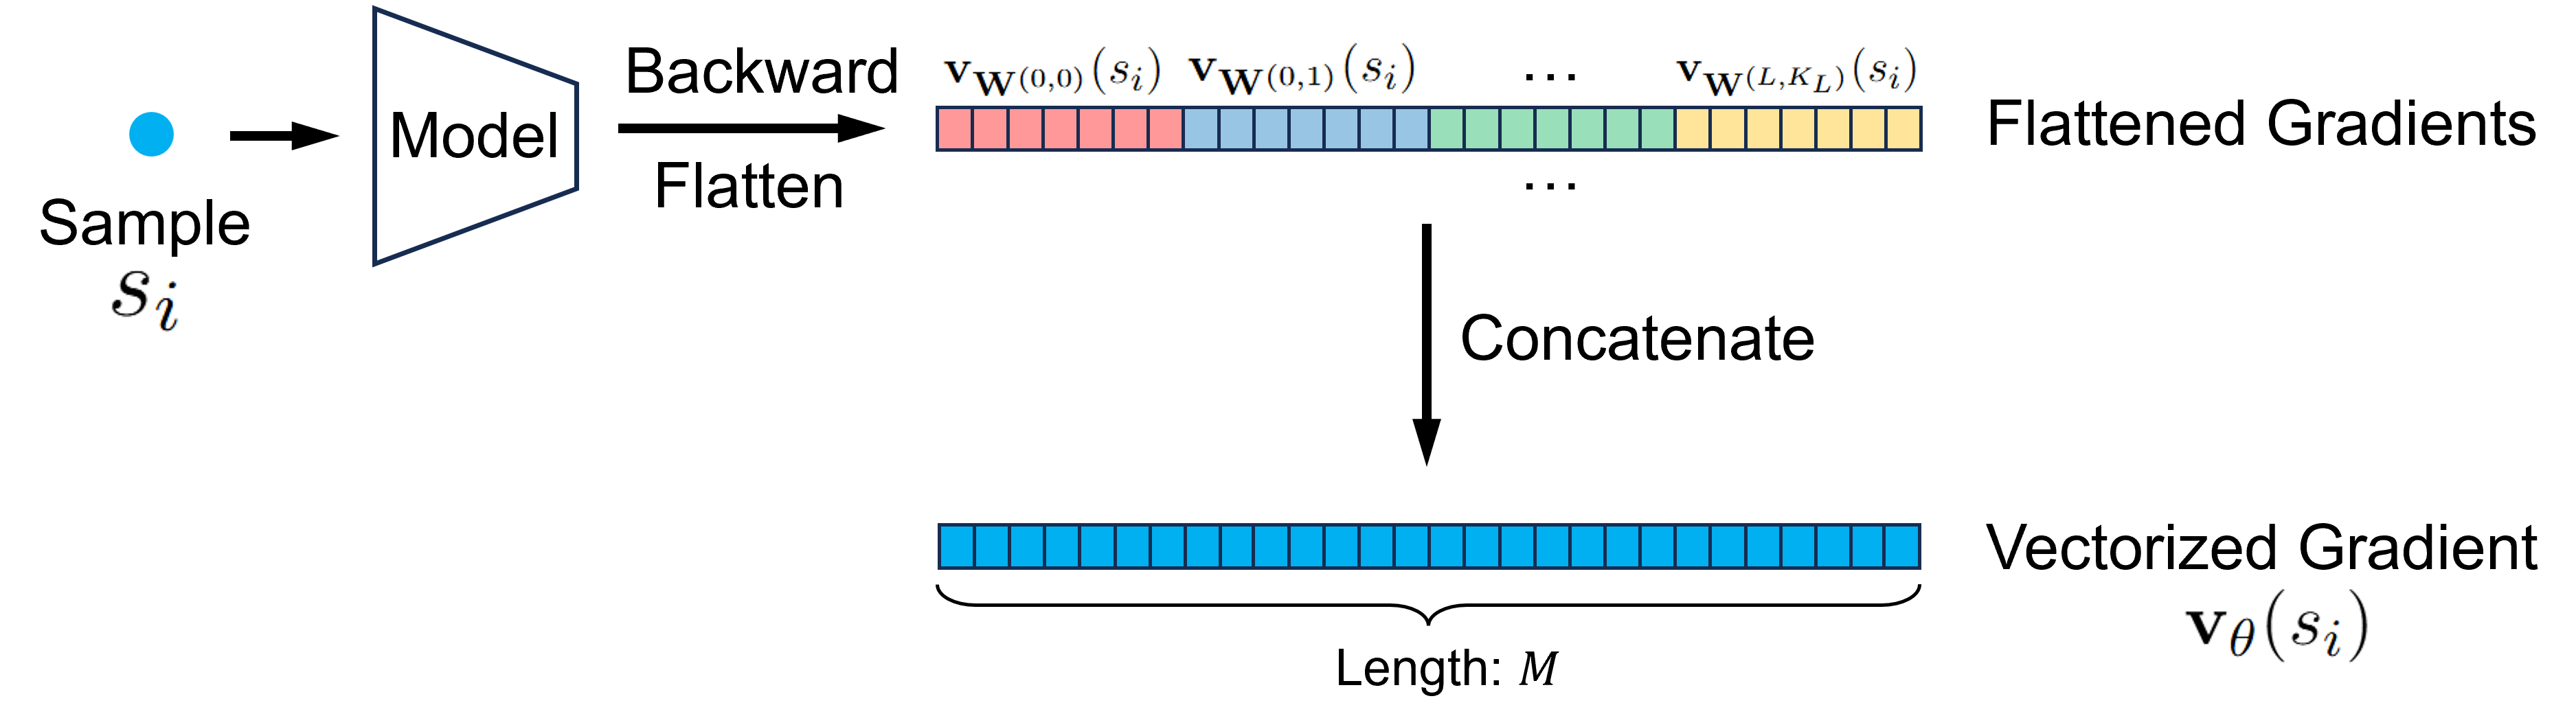
\includegraphics[width=1\textwidth]{figures/gradient_flattening.png}
    \caption{Visual representation of gradient flattening for sample $s_i$.}
    \label{fig:gradient_flattening}
\end{figure}
As a result of the gradient flattening process and the notion of $\vXsi[\theta]$, these vectorized representations of the gradients for different samples can be compared. In other words, the similarity between these can be calculated, which is elaborated in the following section.

\subsection{Similarity Measure}
Generally, a similarity measure is a real-valued function that quantifies the
similarity between two entities.  There are many different ways to measure the
similarity between two mathematical objects such as vectors.  Norms can be used
to measure the distance between two points in space, for example, the $L_1$-
and the $L_2$-norm, called the Manhattan and Euclidean norms, respectively.
Another way of measuring the similarity between two vectors is the dot product.

\subsubsection{Magnitude versus Direction}
The standard dot product between two non-zero vectors
$\mathbf{a},\mathbf{b}\in\mathbb{R}^d$ is defined as
\begin{align*}
    \mathbf{a}^{\top}\mathbf{b}
    \;=\;
    \|\mathbf{a}\|\,\|\mathbf{b}\|\cos{\varphi},
\end{align*}
where $\varphi$ denotes the angle between them. Consequently, a large dot product can arise in two distinct ways:
\begin{enumerate}
    \item \textbf{Directional alignment}: If $\varphi$ is small (for example, $\cos{\varphi} \approx 1$), the vectors point in nearly the same direction and therefore encode similar information.
    \item \textbf{Magnitude imbalance}: Even when $\varphi$ is close to $90^{\circ}$ (poor alignment), the product can still be large if either $\|\mathbf{a}\|$ or $\|\mathbf{b}\|$ is large.
\end{enumerate}
The magnitude of computed gradients from a training set can vary greatly~\cite{sui2021representer} and sometimes blurs the real influence of the gradients in a training set when comparing their local influence on each other~\cite{barshan2020relatifidentifyingexplanatorytraining}. To isolate direction alone, one typically uses cosine similarity,
\begin{align*}
    \simcos(\mathbf{a},\mathbf{b})
    \;=\;
    \frac{\mathbf{a}^{\top}\mathbf{b}}
         {\|\mathbf{a}\|\,\|\mathbf{b}\|},
\end{align*}
which normalizes both vectors and depends solely on the angle~$\varphi$.

\subsubsection{Implications for gradient-based influence analysis}
Using cosine similarity for gradient comparison has three practical advantages:
\begin{enumerate}
    \item \textbf{Magnitude-invariance}: Two gradients affect the score only through their angle and not by their magnitude.
    \item \textbf{Sensitivity to local influence}: By basically ignoring large norm outliers, cosine similarity prioritizes gradients whose direction truly matches that of the comparing gradient, which is the criterion for local influence~\cite{barshan2020relatifidentifyingexplanatorytraining}.
    \item \textbf{Interpretability}: A score of $+1$ means perfect alignment, $0$ orthogonality, and $-1$ opposition, which provides an intuitive quantity of how similar the gradients are.
\end{enumerate}
In short, cosine similarity isolates geometrically relevant information (direction) while
ignoring the interference factor (magnitude), making it an appropriate choice for
gradient-based influence analysis~\cite{Hammoudeh_2024}.

\section{High Gradient Similarity with Similar Samples}
As already mentioned, the original assumption is that when a model is already trained on sample $\si$, then in the paraphrased setting
\begin{equation}
    \simcos \bigl( \vXspi, \vXsi \bigr) > \simcos \bigl( \vXspi, \vXsj \bigr), \qquad \forall\,j\in\{0,\dots,N\}\setminus\{i\}.
    \label{eq:cosine_similarity_paraphrased}
\end{equation}
That means that the full model gradient of the paraphrased sample $\spi$ is most similar to its original sample $\si$ compared to all other original samples $\sj$. If this is the case, then the gradient-based explanation method is able to find the original data point for its paraphrased equivalent. 
\begin{figure}[ht]
    \centering
    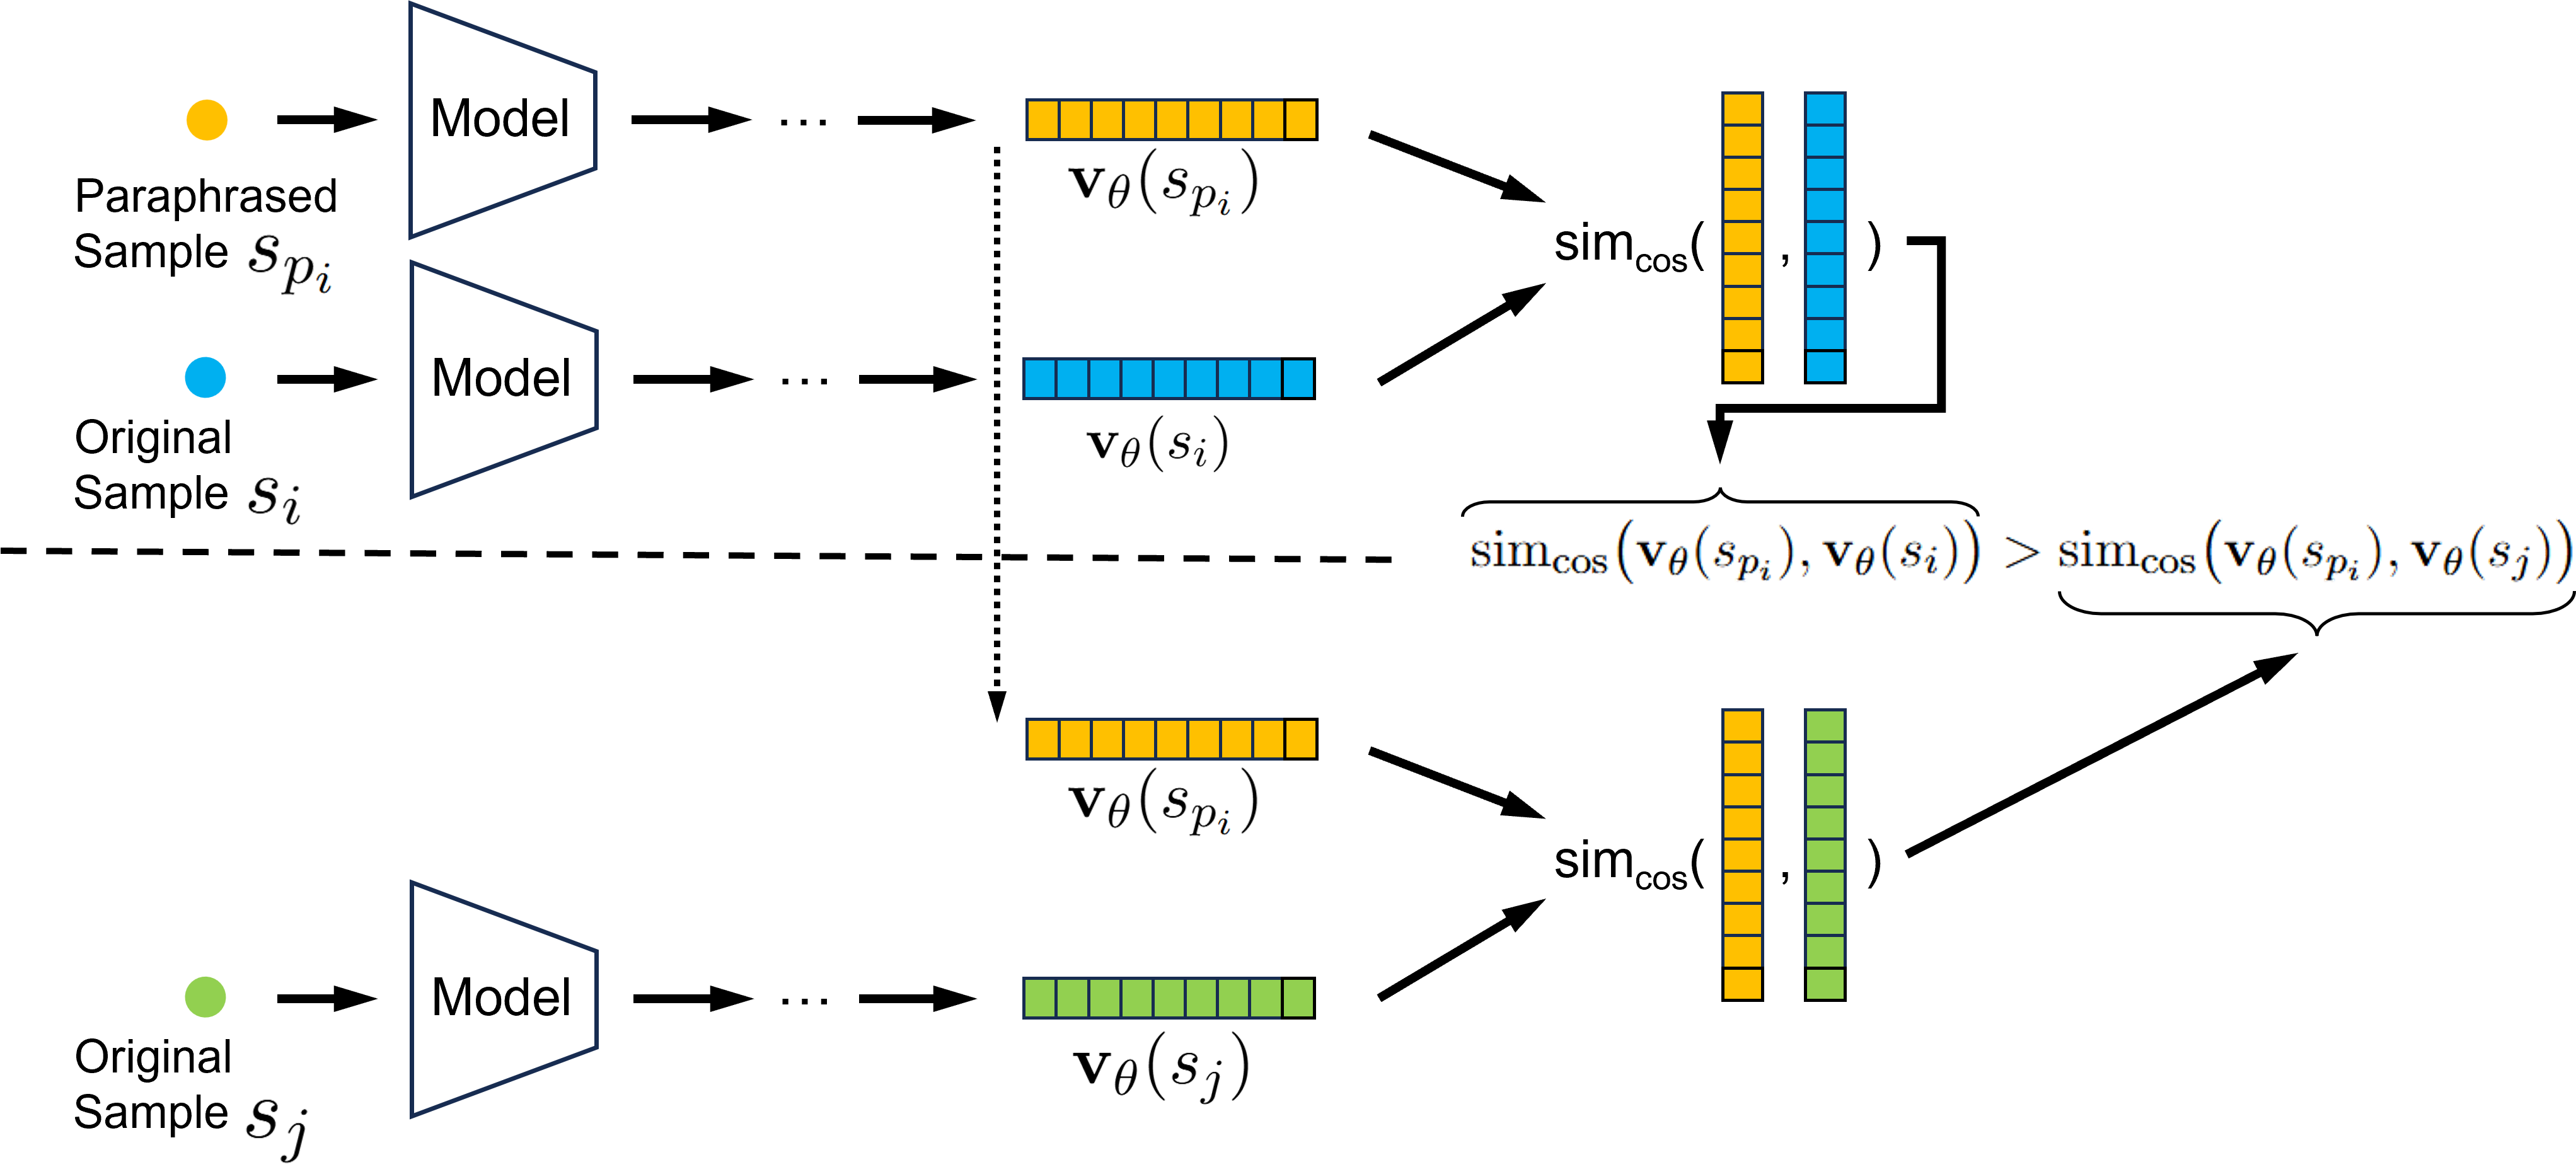
\includegraphics[width=1\textwidth]{figures/gradient_cosine_similarity.png}
    \caption{Visual representation of the gradient cosine similarity comparison between $(\spi, \si)$ and $(\spi, \sj)$.}
    \label{fig:gradient_cosine_similarity}
\end{figure}
For both settings, this comparison is made for all samples $\spi$ and $\smi$ to calculate a score of how well the model gradients can find the equivalent original data points. 
\begin{equation}
\operatorname{accuracy}_\theta(D_p, D)
\;:=\;
\frac{1}{N}\sum_{i=0}^{N}
\bigl[
  \simcos \bigl( \vXspi,\vXsi \bigr)
  \;>\;
  \max_{\substack{j \in 0,1\dots,N  \\j \neq i}}\,
  \simcos \bigl( \vXspi,\vXsj \bigr)
\bigr]
\label{eq:accuracy_full}
\end{equation}
As shown in Equation~\ref{eq:accuracy_full}, when computing $\operatorname{accuracy}_\theta(D_p, D) \in [0,1]$, the gradient for each sample $\si$ and $\spi$ has to be calculated. Due to the high-dimensionality of these gradients in the \acrshort{llm} setting, they cannot be cached in the application's memory nor can they be stored on disk, and hence have to be recomputed for each iteration. More about this is mentioned in Subsection \ref{subsec:high_dimensionality}.

\subsection{BM25-selected Samples}\label{subsec:bm25_selection}
As mentioned above, comparing each paraphrased sample gradient $\spi$ with all original sample gradients $\si$, is computationally very expensive or even practically infeasible for larger models. However, in this setting, it is not necessary to compare each paraphrased sample gradient $\spi$ with the original samples $\si$ from $D$. One could just use a well established ranking function for document retrieval in a text-based setting, in this case BM25~\cite{bm25}. 
\fxnote{Explain what BM25 is and why it is used.}
\fxnote{Explain what $\operatorname{BM25}_D(\spi, \sj)$ regarding corpus $D$, etc. means.}
Algorithm \ref{alg:bm25_select_samples} demonstrates how the $b$ most similar original samples compared to the paraphrased sample $\spi$ are selected and returned using the index set $\mathcal{C}_i(k)$. If the original sample $\si$ is not in the final index set $\mathcal{C}_i(b)$, the least similar sample will be overwritten with it to ensure that the original equivalent of $\spi$ is always present for gradient comparisons.
\begin{algorithm}[ht]
\caption{Retrieve the $b$ Most Similar Original Samples via BM25}
\label{alg:bm25_select_samples}

\KwData{paraphrased sample $\spi$, original dataset $D=\{\si\}_{i=0}^{N}$, desired amount $b$}
\KwResult{$\mathcal{C}_i(b)$ — ordered list of the $b$ most similar original samples compared to paraphrased sample $\spi$}

\DontPrintSemicolon
\For{$j \gets 0$ \KwTo $N$}{
    $\text{score}[j] \gets \operatorname{BM25}_D(\spi, \sj)$\;
}
$\mathcal{C}_i(b) \gets \operatorname{argsort\_topk}(\text{score}, k)$\; \Comment*[r]{The function $\operatorname{argsort\_topk}$ returns the $b$ indices with the highest BM25 scores in descending order and hence, the  samples with the most lexical overlap according to BM25. }

\tcp{Ensure $\mathcal{C}_i(b)$ contains the original sample $\si$ with index $i$}
\If{$i \notin \mathcal{C}_i(b)$}{ 
    $\mathcal{C}_i(b)[k-1] \gets i$ \tcp{overwrite the least-similar (last) entry}
}

\Return $\mathcal{C}_i(b)$
\end{algorithm}
Now that the notion of an index set $\mathcal{C}_i(b)$ with the most lexical overlapping samples to sample $\spi$ is established, the accuracy in Equation~\ref{eq:accuracy_full} can be improved with respect to execution time, as shown in Equation~\ref{eq:accuracy_bm25}. Operationally, restricting each comparison to the BM25 candidate set $\mathcal{C}_i(b)$ removes the all-against-all setting: instead of evaluating $N$ cosine similarities per $\spi$, only $b$ are evaluated. Consequently, the total cost drops from $\mathcal{O}(N^2)$ to $\mathcal{O}(Nb)$ (with $b \ll N$). Additionally, the overwrite rule guarantees that the true pair $(\spi,\si)$ is always present, and only the gradients for these $b$ candidates must be computed or loaded, which further reduces runtime and peak memory.
\begin{equation}
\operatorname{accuracy}^{(b)}_{\theta}(D_{p},D)
\;:=\;
\frac{1}{N}\sum_{i=0}^{N}
\Bigl[
  \simcos\bigl(\vXspi,\,\vXsi\bigr)
  >
  \max_{j\in\mathcal{C}_{i}(b)\setminus\{i\}}
  \simcos\bigl(\vXspi,\,\vXsj\bigr)
\Bigr]
\label{eq:accuracy_bm25}
\end{equation}
The accuracy of the selected samples of BM25 in Equation~\ref{eq:accuracy_bm25} is now used in this article to measure how well gradient-based explanations are able to find the corresponding original data points for the paraphrased ones. However, as illustrated in Subsection~\ref{ssec:different_layers_and_components}, \acrshort{llm}s contain many components that contribute to a full model gradient. Therefore, it makes sense to determine how much each individual layer component contributes to this setting. 

\subsection{Layer Component Comparisons}
\fxnote{Elaborate why each layer is investigated}
Equation~\ref{eq:accuracy_bm25}, illustrates the accuracy of the model by selecting samples with BM25 using the full model gradient. To measure how well each individual layer performs in this setting, this accuracy is adapted to use single layer component gradients, as shown in Equation \ref{eq:layer_accuracy_bm25}.
\begin{equation}
  \begin{split}
    \operatorname{accuracy}^{(b)}_{\Wlk}(D_{p},D)
    := \frac{1}{N}\sum_{i=1}^{N}
        \Bigl[\,
          \simcos\bigl(\vXspi[\Wlk],\vXsi[\Wlk]\bigr)
          \\[4pt]            % ←– line break (add extra space if you like)
    \quad>
          \max_{j\in\mathcal{C}_{i}(b)\setminus\{i\}}
          \simcos\bigl(\vXspi[\Wlk],\vXsj[\Wlk]\bigr)
        \Bigr]
  \end{split}
  \label{eq:layer_accuracy_bm25}
\end{equation}
As described in Section~\ref{sec:greedy_layer_selection} below, the cosine similarity of the combined individual layer components will be computed to establish the so-called Greedy-Layer Selection. For simplicity, define the combined gradient vector for two arbitrary layer components $\Wlonekone$ and $\Wltwoktwo$ and sample $\si$ as
\begin{equation}
\vXsi[\{ \Wlonekone, \Wltwoktwo \}]
\;:=\;
\operatorname{col}\bigl( \vXsi[\Wlonekone], \vXsi[\Wltwoktwo] \bigr).
\end{equation}
The cosine similarity is not a linear function due to the norms in the denominator, and therefore
\begin{equation}
    \begin{split}
        \simcos\bigl(\vXspi[\{ \Wlonekone, \Wltwoktwo \}], \vXsi[\{ \Wlonekone, \Wltwoktwo \}] \bigr) & \neq \\
        \simcos\bigl(\vXspi[\Wlonekone], \vXsi[\Wlonekone] \bigr) & \; + \\ \simcos\bigl(\vXspi[\Wltwoktwo], \vXsi[\Wltwoktwo] \bigr) & .
    \end{split}
    \label{eq:cosine_similarity_non_linearity_example}
\end{equation}
In other words, Equation~\ref{eq:cosine_similarity_non_linearity_example} shows that the cosine similarity of combined gradient vectors is not equal to the sum of its individual gradient vectors due to the non-linearity of the cosine similarity. This can be generalized up to the full model gradient, like
\begin{equation}
\begin{split}
    \simcos\bigl(\vXspi,\,\vXsi\bigr) \neq \sum_{l=0}^{L} \sum_{k=0}^{K_l} \simcos\bigl( \vXspi[\Wlk], \, \vXsi[\Wlk] \bigr ).
    \label{eq:cosine_similarity_non_linearity_full}
\end{split}
\end{equation}
Hence, summing up the cosine similarities for some or all individual layer component gradient vectors for $\spi$ and $\si$ does not equal the full model gradient cosine similarity of $\spi$ and $\si$. Therefore, working directly with the cosine similarity does not suit the setting if gradient vectors of multiple layer components need to be combined. 

\subsubsection{Linearity of the Dot product for Gradient Vectors}
The dot product is \emph{bilinear}, i.e.\ linear in each of its arguments.
For arbitrary vectors $\mathbf{u},\mathbf{v},\mathbf{w}\in\mathbb{R}^d$ and
scalars $\alpha,\beta\in\mathbb{R}^d$
\begin{equation}
  (\alpha\mathbf{u}+\beta\mathbf{v})^{\top}\mathbf{w}
  \;=\;
  \alpha\,\mathbf{u}^{\top}\mathbf{w}
  \;+\;
  \beta\,\mathbf{v}^{\top}\mathbf{w}.
  \label{eq:dot_bilinear}
\end{equation}
Because the collector operator $\operatorname{col}(\cdot)$ stacks the sub‑vectors corresponding to each layer component gradient without overlap and the linearity of the dot product, the dot product between two flattened gradients decomposes into a sum of dot products over the individual components:
\begin{equation}
  \vXspi^{\top}\,\vXsi
  \;=\;
  \sum_{l=0}^{L}\;
  \sum_{k=0}^{K_l}
    \vXspi[\Wlk]^{\top}\,
    \vXsi[\Wlk].
  \label{eq:dot_grad_decompose}
\end{equation}

\subsubsection{Cosine Similarity via Dot Products}
Recall that the $L_2$‑norm of any vector can be expressed as the square root of a self‑dot product:
$\|\mathbf{a}\|=\sqrt{\mathbf{a}^{\top}\mathbf{a}}$.
Consequently, cosine similarity is based on nothing more than dot products. For the \emph{full‑model} gradients of the paraphrased sample~$\spi$ and its original counterpart~$\si$ we obtain
\begin{equation}
\begin{split}
      \simcos\bigl(\vXspi,\vXsi\bigr)
  \;=\;
  \frac{\vXspi^{\top}\vXsi}
       {\sqrt{\vXspi^{\top}\vXspi}\,
        \sqrt{\vXsi^{\top}\vXsi}}\\[12pt]
  \;=\;
  \frac{\displaystyle
        \sum_{l=0}^{L}\sum_{k=0}^{K_l}
        \vXspi[\Wlk]^{\top}\vXsi[\Wlk]}
       {\displaystyle
        \sqrt{\sum_{l=0}^{L}\sum_{k=0}^{K_l}
               \vXspi[\Wlk]^{\top}\vXspi[\Wlk]}\;
        \sqrt{\sum_{l=0}^{L}\sum_{k=0}^{K_l}
               \vXsi[\Wlk]^{\top}\vXsi[\Wlk]}}.
\end{split}
\label{eq:cosine_dot_full}
\end{equation}
The numerator in Equation~\ref{eq:cosine_dot_full} captures the \emph{directional alignment} of the two gradients, while the denominator normalizes by their magnitudes. Consequently, for a single layer component $\Wlk$
\begin{equation}
  \simcos\bigl(\vXspi[\Wlk],\vXsi[\Wlk]\bigr)
  \;=\;
  \frac{\vXspi[\Wlk]^{\top}\vXsi[\Wlk]}
       {\sqrt{\vXspi[\Wlk]^{\top}\vXspi[\Wlk]}\,
        \sqrt{\vXsi[\Wlk]^{\top}\vXsi[\Wlk]}}.
  \label{eq:cosine_dot_layer}
\end{equation}
More generally, let $\mathcal{S}\subseteq \bigl\{\,\Wlk \;\big|\;0\le l\le L,\;0\le k\le K_l\bigr\}$ denote an arbitrary set of layer components. Collecting the corresponding gradient sub-vectors with
$\operatorname{col}(\cdot)$ and applying the same reasoning yields
\begin{equation}
  \simcos\bigl(\vXspi[\mathcal{S}],\vXsi[\mathcal{S}]\bigr)
  \;=\;
  \frac{\vXspi[\mathcal{S}]^{\top}\vXsi[\mathcal{S}]}
       {\sqrt{\vXspi[\mathcal{S}]^{\top}\vXspi[\mathcal{S}]}\,
        \sqrt{\vXsi[\mathcal{S}]^{\top}\vXsi[\mathcal{S}]}}.
  \label{eq:cosine_dot_subset}
\end{equation}
These reformulations show that the cosine similarity can always be evaluated by using dot products. This observation is utilized in the following Section~\ref{sec:greedy_layer_selection}, where the gradients of selected layer components are incrementally combined. Additionally, these intermediate dot products can be easily stored on the disk and later be picked up for further analysis. This is briefly described in Section~\ref{subsec:intermediate_results}.

\section{Greedy Layer Selection (Forward)}\label{sec:greedy_layer_selection}
\fxnote{Introduce general idea and why it is interesting}
\fxnote{Explain why forward greedy selection is preferred instead of backward ...}
The aim of this section is to select, \emph{greedily and forward}, a sequence of layer components whose \emph{combined} gradients best reproduce the full–model cosine similarities
$\gamma_{i,j}^{\theta} = \simcos\bigl(\vXspi,\vXsj\bigr)$ between all paraphrased–original sample pairs.

\subsection{Prerequisites and Notation}\label{ssec:gls_prereq}
Let
\[
\mathcal{W} \;=\; \bigl\{\, (l,k) \;\big|\; 0 \le l \le L,\; 0 \le k \le K_l \bigr\}
\]
denote the \emph{index set} of all layer components of the model (cf.\ Section~\ref{ssec:different_layers_and_components}).
For each index pair $(l,k)\in\mathcal{W}$, write $\W^{(l,k)}$ for the corresponding layer component. For every $(l,k) \in \mathcal{W}$ and every paraphrased–original pair $(i,j)$ we assume the following \emph{dot products} are precomputed and stored (Section~\ref{subsec:intermediate_results}):
\begin{equation}
\begin{split}
\delta^{(l,k)}_{i,j} \;&:=\; \vXspi[\Wlk]^{\top}\vXsj[\Wlk],\\
\delta^{(l,k)}_{i,i} \;&:=\; \vXspi[\Wlk]^{\top}\vXspi[\Wlk],\\
\delta^{(l,k)}_{j,j} \;&:=\; \vXsj[\Wlk]^{\top}\vXsj[\Wlk].
\end{split}
\label{eq:layer_dot_products_repeat}
\end{equation}
For any subset $\mathcal{L}\subseteq\mathcal{W}$ of already selected \emph{indices}, define the \emph{accumulated} dot products
\[
D^{\mathcal{L}}_{i,j} := \sum_{(l,k)\in\mathcal{L}}\delta^{(l,k)}_{i,j}, \qquad
D^{\mathcal{L}}_{i,i} := \sum_{(l,k)\in\mathcal{L}}\delta^{(l,k)}_{i,i}, \qquad
D^{\mathcal{L}}_{j,j} := \sum_{(l,k)\in\mathcal{L}}\delta^{(l,k)}_{j,j}.
\]
Using only the components with indices in $\mathcal{L}$, the \emph{reconstructed} cosine similarity between $\spi$ and $\sj$ is
\begin{equation}
\hat{\gamma}^{\mathcal{L}}_{i,j}
\;:=\;
\frac{D^{\mathcal{L}}_{i,j}}
     {\sqrt{D^{\mathcal{L}}_{i,i}}\,
      \sqrt{D^{\mathcal{L}}_{j,j}}}.
\label{eq:reconstructed_cosine}
\end{equation}
Let $\Gamma^\theta \in \mathbb{R}^{P}$ be the vector that \emph{stacks} all full‑model cosine similarities $\gamma_{i,j}^{\theta}$ for every fixed ordering of the $P$ paraphrased–original pairs $(i,j)$, and let $\hat{\Gamma}^{\mathcal{L}} \in \mathbb{R}^{P}$ stack the reconstructed values $\hat{\gamma}^{\mathcal{L}}_{i,j}$ in the  emph{same} order. In this case $P = N \cdot b$, the number of paraphrased samples times the number of $b$ BM25 selected original samples. As our \emph{goodness (objective) score} for a candidate set $\mathcal{L}$ we use the cosine similarity between these two vectors:
\begin{equation}
\rho(\mathcal{L}) \;:=\;
\simcos\bigl(\hat{\Gamma}^{\mathcal{L}}, \Gamma^\theta\bigr).
\label{eq:rho_objective}
\end{equation}

\paragraph{Goal.}
Starting from $\mathcal{L}_0=\varnothing$, we seek an \emph{ordering} of index pairs
$\bigl((l_1,k_1), (l_2,k_2), \dots\bigr)$ picked one by one such that the running score
$\rho(\mathcal{L}_t)$ improves as quickly as possible:
\[
\mathcal{L}_{t+1} \;=\; \mathcal{L}_t \cup \bigl\{(l^\star,k^\star)\bigr\}
\quad\text{with}\quad
(l^\star,k^\star) \in \arg\max_{(l,k)\in\mathcal{W}\setminus\mathcal{L}_t}
\rho\bigl(\mathcal{L}_t \cup \{(l,k)\}\bigr).
\]

\subsection{Algorithm}\label{subsec:gls_algo}
The forward greedy strategy below maintains the accumulators
$D^{\mathcal{L}}_{i,j}$, $D^{\mathcal{L}}_{i,i}$, $D^{\mathcal{L}}_{j,j}$ (vectorized over all pairs $(i,j)$) and
updates them \emph{once per newly selected index $(l,k)$}. This avoids re‑summing all previously
selected indices at every step (turning a naive $\mathcal{O}(tP)$ re‑sum into
$\mathcal{O}(P)$ per iteration).
\begin{algorithm}[htb]
\caption{Forward Greedy Layer Selection}
\label{alg:greedy_layer_selection}
\DontPrintSemicolon
\KwData{
\begin{tabular}{@{}l@{}}
Precomputed layer dot products 
$\bigl\{\delta^{(l,k)}_{i,j}, \delta^{(l,k)}_{i,i}, \delta^{(l,k)}_{j,j}\bigr\}$\\
Full‑model cosine similarities $\gamma_{i,j}^{\theta}$ for all $(i,j)$\\
A fixed ordering of pairs $(i,j)$ giving vectors of length $P$
\end{tabular}
}
\KwResult{Ordered list $\bigl[((l_1,k_1), \rho_1), \dots, ((l_{|\mathcal{W}|},k_{|\mathcal{W}|}), \rho_{|\mathcal{W}|})\bigr]$}

\BlankLine
\textbf{Flatten} all $(i,j)$ into a fixed list and build $\Gamma^\theta\in\mathbb{R}^P$.\;
\textbf{Normalize} $\Gamma^\theta$ once: $n_\theta \gets \|\Gamma^\theta\|_2$.\;

\BlankLine
\textbf{Initialize accumulators} $D_{ij} \gets \mathbf{0}\in\mathbb{R}^P$,
$D_{ii} \gets \mathbf{0}\in\mathbb{R}^P$,
$D_{jj} \gets \mathbf{0}\in\mathbb{R}^P$.\;
$\mathcal{L}\gets\varnothing$,\quad $\mathcal{R}\gets\mathcal{W}$ (remaining indices),\quad $\varepsilon>0$.\;

\For{$t \gets 1$ \KwTo $|\mathcal{W}|$}{
  $\rho^\star \gets -\infty$, \quad $(l^\star,k^\star)\gets\text{None}$.\;
  \ForEach{$(l,k) \in \mathcal{R}$}{
    \tcp{Propose adding index $(l,k)$}
    $\widetilde{D}_{ij} \gets D_{ij} + \delta^{(l,k)}_{i,j}$\;
    $\widetilde{D}_{ii} \gets D_{ii} + \delta^{(l,k)}_{i,i}$\;
    $\widetilde{D}_{jj} \gets D_{jj} + \delta^{(l,k)}_{j,j}$\;
    \tcp{Vectorized reconstruction of Equation~\ref{eq:reconstructed_cosine}}
    $\hat{\Gamma} \gets \widetilde{D}_{ij} \oslash \bigl(\sqrt{\widetilde{D}_{ii}}\odot \sqrt{\widetilde{D}_{jj}} + \varepsilon\bigr)$\;
    $n \gets \|\hat{\Gamma}\|_2 + \varepsilon$\; \fxnote{change notion of epsilon here, and explain in the text}
    \tcp{Score of Equation~\ref{eq:rho_objective}}
    $\rho \gets \frac{\langle \hat{\Gamma}, \Gamma^\theta \rangle}{n \cdot n_\theta}$\;
    \If{$\rho > \rho^\star$}{
        $\rho^\star \gets \rho$, \quad $(l^\star,k^\star)\gets(l,k)$\;
        $D^\star_{ij}\gets \widetilde{D}_{ij}$, $D^\star_{ii}\gets \widetilde{D}_{ii}$, $D^\star_{jj}\gets \widetilde{D}_{jj}$\;
    }
  }
  \tcp{Commit best index of this round}
  $D_{ij}\gets D^\star_{ij}$,\quad $D_{ii}\gets D^\star_{ii}$,\quad $D_{jj}\gets D^\star_{jj}$\;
  $\mathcal{L}\gets \mathcal{L}\cup\{(l^\star,k^\star)\}$,\quad
  $\mathcal{R}\gets \mathcal{R}\setminus\{(l^\star,k^\star)\}$\;
  \textbf{Store} $((l^\star,k^\star), \rho^\star)$ in the output list.\;
  \tcp{Optional early stop: if $\rho^\star$ saturates or $t$ reaches desired budget}
}
\Return ordered list.
\end{algorithm}

\subsubsection{Complexity}
Let $L_\text{tot}=|\mathcal{W}|$ be the number of (layer) index pairs and $P$ the number of paraphrased–original pairs with $b$ BM25 selected original samples. Each greedy iteration scans all remaining indices and performs $\mathcal{O}(P)$ vector operations, yielding a worst‑case complexity of $\mathcal{O}(L_\text{tot}^2 P)$. In practice, such greedy algorithms usually stop when the objective, in this case $\rho$ plateaus. However, for the sake of completeness, early stopping is not applied to gather more insights on how the algorithm performs with increasing dimensions.

\subsubsection{Numerical Details}
The implementation adds a very small $\varepsilon$ in denominators to avoid divisions by zero and uses vectorization to (i) avoid deep dictionary lookups inside the greedy loop and (ii) keep the per‑iteration cost proportional to $P$.

\subsubsection{Variants}
Besides \emph{forward} selection, one could also do \emph{backward} elimination (start with all indices and iteratively remove the least helpful one) or \emph{beam} search over small subsets. Forward selection is cheaper here because we can re‑use the running accumulators $(D_{ij},D_{ii},D_{jj})$ and never need to re‑materialize full model‑sized vectors. Additionally, the focus is on small vector representations and therefore, the early results of the forward greedy-layer-selection are more interesting for this use case.

\subsection{Random Projection as a Baseline}\label{subsec:random_projection_as_a_baseline}
To validate that the Greedy Layer Selection algorithm identifies a genuinely influential subset of layer components, its performance is compared with a random projection baseline. This baseline helps to answer the question: Does the greedy method significantly outperform a random selection of an equivalent number of parameters?
\\\\
The \acrfull{jl} lemma suggests that even a random projection can preserve the geometry of the data, making it a non-trivial benchmark \cite{johnson_lindenstrauss}. In this context, the baseline is constructed by projecting the entire gradient vector into a lower-dimensional space. The full, high-dimensional gradient vector for a sample $s_i$ is denoted by $\vXsi[\theta] \in \mathbb{R}^M$. A random projection matrix $\mathbf{R} \in \mathbb{R}^{d \times M}$, where $d \ll M$, is used to map this gradient to a lower-dimensional space. The projected gradient vector, $\mathbf{p}(s_i) \in \mathbb{R}^d$, is defined as:
\begin{equation}
    \mathbf{p}(s_i) := \frac{1}{\sqrt{d}} \mathbf{R} \, \vXsi[\theta]
\end{equation}
where $d$ is the target dimension of the projection \cite{rakhshan2022rademacherrandomprojectionstensor}.
\\\\
However, due to computational constraints that prevent materializing the full gradient vector $\vXsi[\theta]$ at once, a layer-wise projection strategy is implemented. For each layer component $\Wlk$, a separate random matrix $\mathbf{R}^{(l,k)} \in \mathbb{R}^{d_{l,k} \times |\Wlk|}$ is used to project the corresponding layer gradient $\vXsi[\Wlk]$, where $d_{l,k}$ is the projection dimension for that layer, proportional to its number of parameters $|\Wlk|$. The final low-dimensional representation is obtained by concatenating these individual projections:
\begin{equation}
    \mathbf{p}(s_i) := \operatorname{col}\left( \frac{1}{\sqrt{d_{0,0}}} \mathbf{R}^{(0,0)} \vXsi[\W^{(0,0)}], \dots, \frac{1}{\sqrt{d_{L,K_L}}} \mathbf{R}^{(L,K_L)} \vXsi[\W^{(L,K_L)}] \right).
\end{equation}
The cosine similarity is then computed between these resulting projected vectors $\mathbf{p}(s_i)$ and $\mathbf{p}(s_j)$ for each sample pair.
\\\\
The comparison is performed as follows:
\begin{enumerate}
    \item The {full-model gradient similarity} is computed for each sample pair $(\spi, \sj)$ to establish a ground truth. This involves calculating the gradient for each sample, flattening the gradient tensors for all layers into a single high-dimensional vector $\vXsi[\theta]$, and then computing the cosine similarity between these flattened vectors.
    \item The Greedy Layer Selection (Algorithm \ref{alg:greedy_layer_selection}) is executed to iteratively build a subset of layer components whose combined gradients best approximate the ground-truth similarities.
    \item A layer-wise random projection of the gradients is performed as a baseline. For each sample, the gradient vector of every individual layer component $\vXsi[\Wlk]$ is projected separately into a lower-dimensional space. These individual projected vectors are then concatenated to form a single, final low-dimensional representation of the full model gradient.
    \item Finally, the cosine similarity is calculated between these concatenated, low-dimensional projected gradient vectors for each sample pair. The results of this baseline are then compared against the ground truth as well. 
\end{enumerate}

\fxnote{maybe mention processess of the jupyter notebook after intermediate results are computed}

\subsection{Greedy Layer Selection by Retrieval Accuracy}\label{subsec:gls_accuracy}
The forward strategy in Section~\ref{sec:greedy_layer_selection} selects layer components by maximizing the cosine similarity between reconstructed and full-model gradient similarities. In many applications, however, the end goal is \emph{retrieval}: for each paraphrased sample $\spi$, identify its original counterpart $\si$ within the BM25 candidate set $\mathcal{C}_i(b)$ (cf.\ Section~\ref{subsec:bm25_selection}). This subsection introduces a complementary greedy procedure that directly optimizes the \emph{top-1 retrieval accuracy} induced by the currently selected layer components.

\subsubsection{Objective}
Recall the per-component dot products $\delta^{(l,k)}_{i,j}$, $\delta^{(l,k)}_{i,i}$, and $\delta^{(l,k)}_{j,j}$ from Equation~\ref{eq:layer_dot_products_repeat}. For a set of selected indices $\mathcal{L}\subseteq\mathcal{W}$, define the accumulated dot products
\[
D^{\mathcal{L}}_{i,j}=\sum_{(l,k)\in\mathcal{L}}\delta^{(l,k)}_{i,j},\qquad
D^{\mathcal{L}}_{i,i}=\sum_{(l,k)\in\mathcal{L}}\delta^{(l,k)}_{i,i},\qquad
D^{\mathcal{L}}_{j,j}=\sum_{(l,k)\in\mathcal{L}}\delta^{(l,k)}_{j,j}.
\]
Using Equation~\ref{eq:reconstructed_cosine}, the cosine similarity reconstructed from the selected components is
\[
\hat{\gamma}^{\mathcal{L}}_{i,j}
\;=\;
\frac{D^{\mathcal{L}}_{i,j}}
     {\sqrt{D^{\mathcal{L}}_{i,i}}\,
      \sqrt{D^{\mathcal{L}}_{j,j}}}.
\]
Restricting comparisons to the BM25 candidate set $\mathcal{C}_i(b)$ (which, by construction, contains $i$), the accuracy attained by $\mathcal{L}$ is
\begin{equation}
\operatorname{accuracy}^{(b)}_{\mathcal{L}}(D_p,D)
\;:=\;
\frac{1}{N}\sum_{i=0}^{N}
\Bigl[
\hat{\gamma}^{\mathcal{L}}_{i,i}
>
\max_{j\in\mathcal{C}_i(b)\setminus\{i\}}
\hat{\gamma}^{\mathcal{L}}_{i,j}
\Bigr].
\label{eq:accuracy_bm25_reconstructed}
\end{equation}
The greedy rule is to add, at each step, the single layer component whose inclusion yields the largest \emph{current} value of Equation~\ref{eq:accuracy_bm25_reconstructed}. As above, all statements apply identically when replacing $\spi$ with $\smi$.

\subsubsection{Algorithm}
The procedure below maintains accumulated dot products over all $(i,j)$ pairs and evaluates the accuracy objective after tentatively adding each remaining component. To ensure well-defined divisions, a small $\varepsilon>0$ is added in denominators.
\begin{algorithm}[htb]
\caption{Forward Greedy Layer Selection by Accuracy}
\label{alg:greedy_layer_selection_accuracy}
\DontPrintSemicolon
\KwData{
\begin{tabular}{@{}l@{}}
BM25 candidate index sets $\{\mathcal{C}_i(b)\}_{i=0}^{N}$ (each $\mathcal{C}_i(b)$ contains $i$)\\
Precomputed per-component dot products $\bigl\{\delta^{(l,k)}_{i,j}, \delta^{(l,k)}_{i,i}, \delta^{(l,k)}_{j,j}\bigr\}$\\
Set of layer indices $\mathcal{W}$, small constant $\varepsilon>0$
\end{tabular}
}
\KwResult{Ordered list $\bigl[((l_1,k_1), a_1), \dots, ((l_{|\mathcal{W}|},k_{|\mathcal{W}|}), a_{|\mathcal{W}|})\bigr]$ of layers and running accuracies}

\BlankLine
\textbf{Initialize accumulators} $D_{i,j}\gets 0$, $D_{i,i}\gets 0$, $D_{j,j}\gets 0$ for all pairs $(i,j)$ with $j\in\mathcal{C}_i(b)$.\;
$\mathcal{L}\gets\varnothing$, \quad $\mathcal{R}\gets\mathcal{W}$ (remaining indices).\;
\For{$t \gets 1$ \KwTo $|\mathcal{W}|$}{
  $a^\star\gets -\infty$, \quad $(l^\star,k^\star)\gets\text{None}$, \quad store best temporary accumulators.\;
  \ForEach{$(l,k)\in\mathcal{R}$}{
    \tcp{Propose adding $(l,k)$ to the selection}
    $\widetilde{D}_{i,j}\gets D_{i,j}+\delta^{(l,k)}_{i,j}$,\quad
    $\widetilde{D}_{i,i}\gets D_{i,i}+\delta^{(l,k)}_{i,i}$,\quad
    $\widetilde{D}_{j,j}\gets D_{j,j}+\delta^{(l,k)}_{j,j}$.\;
    \tcp{Compute reconstructed similarities $\hat{\gamma}^{\mathcal{L}\cup\{(l,k)\}}_{i,j}$}
    $\hat{\gamma}_{i,j}\gets \widetilde{D}_{i,j}\big/\bigl(\sqrt{\widetilde{D}_{i,i}}\sqrt{\widetilde{D}_{j,j}}+\varepsilon\bigr)$ for all $(i,j)$.\;
    \tcp{Evaluate accuracy of Equation~\ref{eq:accuracy_bm25_reconstructed}}
    $a \gets \frac{1}{N}\sum_{i=0}^{N}\Bigl[\hat{\gamma}_{i,i}>\max_{j\in\mathcal{C}_i(b)\setminus\{i\}}\hat{\gamma}_{i,j}\Bigr]$.\;
    \If{$a > a^\star$}{
      $a^\star\gets a$, \quad $(l^\star,k^\star)\gets(l,k)$, \quad save $\widetilde{D}$ as current best.
    }
  }
  \tcp{Commit best index of this round}
  $D_{i,j}\gets \widetilde{D}_{i,j}$,\quad $D_{i,i}\gets \widetilde{D}_{i,i}$,\quad $D_{j,j}\gets \widetilde{D}_{j,j}$.\;
  $\mathcal{L}\gets \mathcal{L}\cup\{(l^\star,k^\star)\}$,\quad
  $\mathcal{R}\gets \mathcal{R}\setminus\{(l^\star,k^\star)\}$.\;
  \textbf{Store} $((l^\star,k^\star), a^\star)$ in the output list.\;
}
\Return ordered list.
\end{algorithm}

\subsubsection{Complexity}
Let $L_\text{tot}=|\mathcal{W}|$ be the number of layer components and $P=\sum_{i}|\mathcal{C}_i(b)|=N\cdot b$ the number of paraphrased–candidate pairs. Each greedy iteration scans all remaining components and performs $\mathcal{O}(P)$ vector operations to update accumulators and evaluate Equation~\ref{eq:accuracy_bm25_reconstructed}, resulting in a worst-case complexity of $\mathcal{O}(L_\text{tot}^2 P)$, analogous to Algorithm~\ref{alg:greedy_layer_selection}.

\subsubsection{Numerical details and ties}
A very small $\varepsilon$ in the denominator prevents divisions by zero. When $D^{\mathcal{L}}_{i,i}D^{\mathcal{L}}_{j,j}\approx 0$, the corresponding $\hat{\gamma}_{i,j}$ is set to a well-defined finite value (e.g.\ zero or $-\infty$ before the comparison), which leaves the top-1 decision unchanged for well-conditioned pairs. Ties in the $\max$ over $j$ are broken deterministically (e.g.\ by index order). As in Section~\ref{subsec:intermediate_results}, storing and re-using component-wise dot products enables efficient recomputation without ever materializing full model-sized gradient vectors.

\subsubsection{Relation to similarity-based selection.}
Whereas Algorithm~\ref{alg:greedy_layer_selection} optimizes the agreement between reconstructed and full-model similarities (a \emph{proxy} for retrieval), Algorithm~\ref{alg:greedy_layer_selection_accuracy} directly optimizes the retrieval objective in Equation~\ref{eq:accuracy_bm25_reconstructed}. The two criteria can favor different components: layers that most closely track global similarity structure need not be those that most improve top-1 decisions within the BM25 candidate sets. In practice, both views are informative and can be reported jointly. 

    \chapter{TBR: Methodology - Experimental Setup}
\fxnote{TODO: introduction text}

\section{HuggingFace as a General Model and Data Provider}
asdf

\subsection{OLMo}
The OLMo model series, developed by the \emph{Allen Institute for AI}, provides open-source \acrshort{llm}s along with their training data and comprehensive training pipelines~\cite{Groeneveld2023OLMo}. These features make OLMo models particularly suitable for research focused on explainability. Specifically, OLMo models are pre-trained on the \emph{Dolma} dataset, which comprises approximately three trillion tokens collected from diverse sources~\cite{dolma}. To adapt these models to specific tasks, the \emph{Open Instruct} framework combined with the \emph{TÜLU} dataset is employed for fine-tuning~\cite{ivison2023camels}.
\\\\
In this article, the focus is on the \texttt{AMD-OLMo-1B-SFT} model from AMD, which is derived from the original \texttt{OLMo-1B} architecture, as detailed in Table~\ref{tab:model_architecture_olmo_1b_amd}. This specific model was pre-trained using the \emph{Dolma v1.7} dataset, consisting of 1.3 trillion tokens, and subsequently fine-tuned through supervised training on the \emph{TÜLU v2} dataset~\cite{AMD-OLMo}.
\begin{table}[htb]
    \centering
    \begin{tabular}{|c|c|c|c|c|c|}
        \hline  
        \BreakHeader{Parameter \\ size} & \BreakHeader{Number of \\ layers} & \BreakHeader{Number of \\ heads} & \BreakHeader{Hidden \\ size} & \BreakHeader{Context \\ length} & \BreakHeader{Vocabulary \\ Size} \\ 
        \hline  
        1.2B & 16 & 16 & 2048 & 20248 & 50280 \\
        \hline
    \end{tabular}
    \caption{Model architecture size of AMD-OLMo-1B-SFT}
    \label{tab:model_architecture_olmo_1b_amd}
\end{table} 
The model is loaded using \emph{HuggingFace}\textquotesingle s \emph{transformers} function \texttt{from\_pretrained(\textless model\textgreater)} from the class \texttt{AutoModelForCausal}, where \texttt{model} is the model name (\texttt{AMD-OLMo-1B-SFT}). It allows published models with corresponding pre-trained weights to be downloaded and further adapted using \emph{PyTorch}. The complete model architecture when loaded with the \emph{transformers} and printed on the console looks like:
\begin{verbatim}
OlmoForCausalLM(
  (model): OlmoModel(
    (embed_tokens): Embedding(50304, 2048, padding_idx=1)
    (layers): ModuleList(
      (0-15): 16 x OlmoDecoderLayer(
        (self_attn): OlmoAttention(
          (q_proj): Linear(in_features=2048, out_features=2048, bias=False)
          (k_proj): Linear(in_features=2048, out_features=2048, bias=False)
          (v_proj): Linear(in_features=2048, out_features=2048, bias=False)
          (o_proj): Linear(in_features=2048, out_features=2048, bias=False)
        )
        (mlp): OlmoMLP(
          (gate_proj): Linear(in_features=2048, out_features=8192, bias=False)
          (up_proj): Linear(in_features=2048, out_features=8192, bias=False)
          (down_proj): Linear(in_features=8192, out_features=2048, bias=False)
          (act_fn): SiLU()
        )
        (input_layernorm): OlmoLayerNorm()
        (post_attention_layernorm): OlmoLayerNorm()
      )
    )
    (norm): OlmoLayerNorm()
    (rotary_emb): OlmoRotaryEmbedding()
  )
  (lm_head): Linear(in_features=2048, out_features=50304, bias=False)
)
\end{verbatim}
As shown above, the model consists of the following trainable components with corresponding dimensionality.
\begin{itemize}
    \item \textbf{Input Embedding:} $\mathbf{E} \in \mathbb{R}^{|V| \times d_x}$
    \item \textbf{16 Decoder Layers ($l = 0, \ldots, 15$):}
    \begin{itemize}
        \item \textbf{Attention:}
        \begin{itemize}
            \item \textbf{Query-Projection:} \hspace{0.6em} $\mathbf{W}_\text{Q}^{(l)} \in \mathbb{R}^{d_x \times d_x}$
            \item \textbf{Key-Projection:} \hspace{1.8em} $\mathbf{W}_\text{K}^{(l)} \in \mathbb{R}^{d_x \times d_x}$
            \item \textbf{Value-Projection:} \hspace{1.3em} $\mathbf{W}_\text{V}^{(l)} \in \mathbb{R}^{d_x \times d_x}$
            \item \textbf{Output-Projection:} \hspace{0.5em} $\mathbf{W}_\text{O}^{(l)} \in \mathbb{R}^{d_x \times d_x}$
        \end{itemize}
        \item \textbf{MLP:}
        \begin{itemize}
            \item \textbf{Gate-Projection:} \hspace{1.7em} $\mathbf{W}_\text{gate}^{(l)} \in \mathbb{R}^{d_x \times d_{ff}}$
            \item \textbf{Up-Projection:} \hspace{2.3em} $\mathbf{W}_\text{up}^{(l)} \in \mathbb{R}^{d_x \times d_{ff}}$
            \item \textbf{Down-Projection:} \hspace{1.2em} $\mathbf{W}_\text{down}^{(l)} \in \mathbb{R}^{d_{ff} \times d_x}$
        \end{itemize}
    \end{itemize}
    \item \textbf{Output Embedding:} $\mathbf{W}^{(o)} \in \mathbb{R}^{d_x \times |V|}$
\end{itemize}

Explanation for each:

\begin{itemize}
\item $|V|$: Vocabulary size (for \texttt{AMD-OLMo-1B-SFT}, $|V| = 50{,}304$).
\item $d_x$: Hidden size (for \texttt{AMD-OLMo-1B-SFT}, $d_x = 2{,}048$).
\item $d_{ff}$: Feedforward/MLP hidden width (for \texttt{AMD-OLMo-1B-SFT}, $d_{ff} = 8{,}192$).
\end{itemize}


\fxnote{maybe go more into the detail of the architecture regarding weights, activation function, etc.}
\fxnote{reference model size equation from previous chapter and establish detailed model size}
\fxnote{list all layers with their corresponding sizes}

\subsection{LIMA Dataset}\label{subsec:lima_dataset}
The \emph{LIMA} dataset is a subset of the \emph{TÜLU} dataset, containing 1,000 carefully curated prompts and responses across various domains, including STEM fields, alongside manually authored samples \cite{zhou2023limaalignment}. Similar to other instruction-tuning datasets, it comprises pairs of prompts and corresponding generations. A prompt typically represents a user's instruction or query, specifying the task or information the model should provide. The model's output, referred to as a generation or response, directly addresses the user's prompt. An illustrative example from the \emph{LIMA} dataset is provided below. This example shows how much quality and depth the \emph{LIMA} dataset has. In this case, the example is well-referenced and closely resembles an expert-level response.
\\\\
User prompt $s_{0_P}$:
\begin{verbatim}
    Can brain cells move? By movement I mean long distance migration 
    (preferably within the brain only).
\end{verbatim}
Model-generation $s_{0_G}$:
\begin{verbatim}
    The question is relatively broad and one should take into account that 
    the brain not only consists of neurons, but also glial cells 
    (supportive cells) and pre-mitotic neuronal stem cells. Furthermore,
    as critical fellow-scientists have indicated, developmental stage is
    very important, as the developing embryonic brain is very different 
    from the adult brain.\nHowever, after sifting through various 
    publications, the answer to the question is actually remarkably 
    simple: Yes, brain cells migrate.\nIn  the adult brain glial cells
    migrate in the brain (Klämbt, 2009). Glial cells are involved in a
    myriad of functions, but a notable example of migrating glial cells
    are the oligodendrocytes that migrate relative long distances to 
    find their target axons onto which they wrap themselves to form the
    insulating myelin sheath (Tsai and Miller, 2002).\nNeuronal stem cells
    migrate over long distances in response to injury (Imitola et al., 2004)
    and they migrate from specific stem-cell locations (e.g., hippocampus 
    and subventricular zone) to other regions (Clarke, 2003).\nPost-mitotic,
    but non-differentiated neurons have been shown to migrate in the adult 
    brain in fish (Scott et al., 2012), and in mammals and non-human 
    primates as well (Sawada et al., 2011).\nNot surprisingly, glial cells, 
    stem cells and neurons also migrate during embryonic development. 
    Most notably, post-mitotic neurons destined to fulfill peripheral 
    functions have to migrate over relatively long distances from the 
    neural crest to their target locations (Neuroscience, 2nd ed, 
    Neuronal Migration).
\end{verbatim}

\section{Preparing the Data}
A small portion of the examples contain complete dialogues with multiple prompts and corresponding responses. These are removed from the dataset to keep the classic prompt/generation theme for all examples and to make them comparable. When removing those dialogue examples, the filtered dataset still consists of $N = 988$ query/response pairs.

\subsection{User/Assistant Message Format}\label{subsec:message_format}

\subsubsection{General Overview}
To ensure consistency and compatibility with modern conversational AI frameworks, each example in the dataset is represented as a list of message objects. Every message specifies both a \texttt{role}, indicating whether it originates from the user, the assistant, or optionally the system, and a \texttt{content} field containing the text.As stated previously, the dialogue examples have been filtered to retain exactly one user-assistant exchange per sample, enforcing a single-turn instruction-response structure for all pairs.

\subsubsection{Roles and Their Purpose}
\begin{itemize}
\item \textbf{system}: An optional message that provides general context or high-level instruction, such as persona or tone guidelines.
\item \textbf{user}: Represents the prompt or question, serving as the input for which the model must generate a response.
\item \textbf{assistant}: Contains the model's response to the user's prompt; this serves as the target output during both training and evaluation.
\end{itemize}

\subsubsection{Dataset Schema}
Each data point is stored in JSON format as a dictionary with a single \texttt{messages} key, which holds a list of message objects. A typical single-turn user-assistant interaction is structured as follows:
\begin{lstlisting}[caption={User–assistant message pair}]
{"messages": [
    { "role": "user", "content": "<query>" },
    { "role": "assistant", "content": "<model output>" }
]}
\end{lstlisting}
This uniform structure facilitates both supervised fine-tuning and later evaluation using the same message format.

\subsection{Paraphrasing Samples}\label{sec:paraphrasing_samples}
As already mentioned in Section~\ref{sec:paraphrasing_a_dataset}, the covered approach operates with two different settings, namely \emph{paraphrased} and \emph{model-generated} paraphrasing levels. For the \emph{paraphrased} case, both the query (user message) and the generation (assistant message) are altered using \emph{OpenAI GPT-4o-mini} with a seed of $42$ and a temperature of $1$. The rest of the parameters are set to default values. The corresponding system prompt is illustrated below:
\begin{verbatim}
    You are a paraphrasing expert who is specialized in rewriting text 
    (questions, statements, etc.) without altering the content. 
    Keep in mind, that the meaning must not change after the paraphrasing. 
    Just output the paraphrased text without any additional information.
\end{verbatim}
The \emph{OpenAI} API also follows the message format shown in Subsection~\ref{subsec:message_format}. Consequently, when paraphrasing the example from Subsection~\ref{subsec:lima_dataset}, the \emph{OpenAI} API receives a system-user message pair object containing the previously illustrated system prompt and the text to be rephrased. Hence, all the samples and therefore, each user and assistant message from the filtered \emph{LIMA} dataset are individually sent to \emph{OpenAI} to be paraphrased. For example, the paraphrase of the the user message prompt shown in Subsection~\ref{subsec:lima_dataset} looks like:
\begin{verbatim}
    Are brain cells capable of moving? Specifically, I’m referring to
    long-distance migration, ideally occurring within the brain.
\end{verbatim}
Section~\ref{subsec:appendix_paraphrased_sample} additionally illustrates the paraphrases for the messages shown in Subsection~\ref{subsec:lima_dataset}. This procedure is then repeated for all samples $\si$ in $D$ to create the dataset $D_p$ first mentioned in Section~\ref{sec:paraphrasing_a_dataset}. To create the dataset $D_m$ for the \emph{model-generated} case, the paraphrased user messages from $D_p$ are input to the model under evaluation. For each paraphrased user message $s_{p_{i_P}}$, the model generates a new assistant message $s_{m_{i_G}}$.

\subsection{Prepare Model-generated Data Point}\label{subsec:prepare_model_input}
Before the user message can be picked up by the model, some modifications are made to the sample. Usually, the user message is embedded inside a form of tag that tells the model where the user message starts and ends. How these tags are formatted and applied differs from model to model in the corresponding training pipeline. In the case of \texttt{AMD-OLMo-1B-SFT}, it looks like:
\begin{verbatim}
    <|user|>\n
    Are brain cells capable of moving? 
    Specifically, I'm referring to long-distance migration, 
    ideally occurring within the brain.\n
    <|assistant|>\n
\end{verbatim}
The \texttt{<|user|>} tag tells the model where the user message starts. The \texttt{<|assistant|>} tag tells the model where the user message ends and that the model should start writing the response. In the space of HuggingFace, this kind of format is usually called \emph{chat template}. After applying this template, the text is tokenized and converted to a numerical format by a so-called \emph{tokenizer} to make it readable for the model. For \texttt{AMD-OLMo-1B-SFT}, the tokenized and converted sequence looks like the following:
\begin{verbatim}
     29, 93, 4537, 49651, 187, 6723, 3998, 1341, 7032, 273,
     4886, 32, 13658, 13, 309, 1353, 14339, 281, 1048, 14,
     19893, 10346, 13, 34243, 12952, 1561, 253, 3998, 15, 187,
     29, 93, 515, 5567, 49651, 187
\end{verbatim}
Each number represents one token; for example, the value $187$ encodes the term \texttt{\textbackslash n}. This sequence of tokens is used to generate a response, which also represents a sequence of tokens. This sequence is then decoded using the same \emph{tokenizer} as before. Section~\ref{subsec:appendix_model_generated_sample} illustrates the decoded answer for the example shown above.
\\\\
This process is then repeated for each original sample to generate the \emph{paraphrased} dataset $D_p$ and the \emph{model-generated} dataset $D_m$. These \emph{paraphrased} and \emph{model-generated} examples are stored on disk and picked up when needed to guarantee a level of determinism when operating on this newly created dataset. 
\fxnote{can I mention my own github repo? Maybe I can publish the dataset on HuggingFace and mention it here}

\subsection{Supervised Fine-Tuning Setup}
Although no additional \acrfull{sft} is performed in this work, all data samples are prepared according to established \acrshort{sft} conventions. This ensures full compatibility with existing model evaluation pipelines and facilitates the subsequent analysis of model behavior from an explainability perspective. Specifically, each sample is formatted as a user–assistant message pair, following the schema described in previous sections.
\\\\
\acrfull{sft} is a process in which a pretrained language model is further trained on a collection of task-specific examples, each consisting of an input (such as a user prompt) and an expected output (such as an assistant response). The goal is to optimize the model’s parameters so that its outputs closely match the ground truth responses, typically minimizing loss of cross-entropy. In the context of conversational models, \acrshort{sft} datasets are structured as lists of message objects, each message specifying a \texttt{role} (e.g., user or assistant) and a \texttt{content} field, as described in Section~\ref{subsec:message_format}. Formatting the data in this standardized way enables the fine-tuning process to teach the model not only to generate accurate responses, but also to adhere to the required conversational structure. As already mentioned, no further \acrshort{sft} is performed in this work, but all samples are formatted in this way to ensure full compatibility with existing pipelines and to support consistent evaluation.

\subsubsection{Open-Instruct}
In the context of this work, \emph{Open-Instruct} is mainly utilized to preprocess and structure the data according to established \acrshort{sft} conventions. Specifically, the framework offers utilities for converting raw user–assistant-message pairs such as those from the \emph{LIMA} dataset into the standardized chat template format (e.g., \texttt{<|user|>} and \texttt{<|assistant|>} tags) used by models like \texttt{AMD-OLMo-1B-SFT}. This ensures consistency between the data preparation procedure and the input expectations of the underlying model architecture.
\\\\
To preprocess the data for \acrfull{sft}, \emph{SFTDatasetProcessor} from \emph{Open-Instruct} is used. It allows a whole dataset to be tokenized and prepared by forming the corresponding input and output sequences and naturally integrating into the \emph{HuggingFace} ecosystem for \acrshort{sft}.

\section{Instance- and Gradient-based Explanation}
\fxnote{mention batch size of 1}

\subsection{High Dimensionality}\label{subsec:high_dimensionality}
\fxnote{mention gradient caching on disk and why it's not suitable for our case, also calculate potential disk usage}

\subsection{BM25-selected Samples}\label{subsec:setup_bm25}
\fxnote{explain that by comparing the first 20 gradients NxN, the most similar examples where in the main diagonal}
\fxnote{reduce execution time by selection top-n BM25 selected samples}

\subsection{Intermediate Results}\label{subsec:intermediate_results}

\fxnote{dot products (per layer) as intermediate results to compute gradient cosine similarity later on because full gradients have to be stored for each sample and each gradient is as big as the model size}

\fxnote{add execution times, server resources, etc.}
    \chapter{Methodology - Results / Is the Full Model Gradient a good Baseline?}
results comparing paraphrased setting and model generated setting

\fxnote{also include heatmap of similar gradients in results sections}

\section{Performance of Gradient-Similarity as an Explanation Method}
asdf

\section{Single Layer Performance}
\fxnote{how "well" does each layer find the most relevant sample to paraphrased samples}

\section{Comparison of Layer-Gradients and Full-Model-Gradients}
\fxnote{Which layers are most similar to the full-gradient, e.g. MLP, ATTN, Embeddings?}

\section{Greedy-Forward-Layer-Selection vs. Random Projections}
asdf
    \chapter{Discussion}

\section{Layer Analysis}
\fxnote{Analyze layer in terms of dimensionality, location, etc. and why they contribute what they contribute}

\section{Comparison}
\fxnote{comparison of random projections, layer selection, etc.}
\fxnote{How do the findings relate to the current literature in regard to layer selection}
    \chapter{Conclusion}
asdf

\section{Future Outlook}
asdf
    
	%add your sources in the bib file and change the style here
    \bibliographystyle{alpha}
	\bibliography{bibliography}

        \noindent ChatGPT and Writefull were used to rephrase sentences or words to make the language, tonality, and writing style more coherent and easier to read.
	
	\printglossary[type=\acronymtype]
    \printglossary

    \cleardoublepage{}\pagebreak
	
	%add your end matter here
	\appendix{}

	\chapter{Appendix}
\section{Nomenclature}
\begin{table}[htb]
    \centering
    \begin{tabular}{ll}
        $\theta_0$ & Model parameters at the start of training \\ 
        $\theta_T$ & Model parameters at the end of training \\
    \end{tabular}
    \caption{General nomenclature reference}
    \label{tab:nomenclature}
\end{table}

\section{AMD-OLMo-1B-SFT}
The number of parameters as a horizontal bar graph is shown in Figure~\ref{fig:parameters_per_layer_amd_olmo}.
\begin{figure}[ht]
    \centering
    
\includegraphics[width=0.63\textwidth]{figures/parameters_per_layer.png}
    \caption{Visual representation of the parameters per layer component for model \texttt{AMD-OLMo-1B-SFT}}
    \label{fig:parameters_per_layer_amd_olmo}
\end{figure}

\section{Preliminary Analysis of Gradient Dot Products}
A preliminary analysis of gradient dot products between $25$ paraphrased and original samples is shown in Figure~\ref{fig:preliminary_analysis_dot_products}. As illustrated there, the main diagonal contains significantly higher values, indicating that the model is able to find the corresponding original data points. 

\begin{figure}[ht]
    \centering
    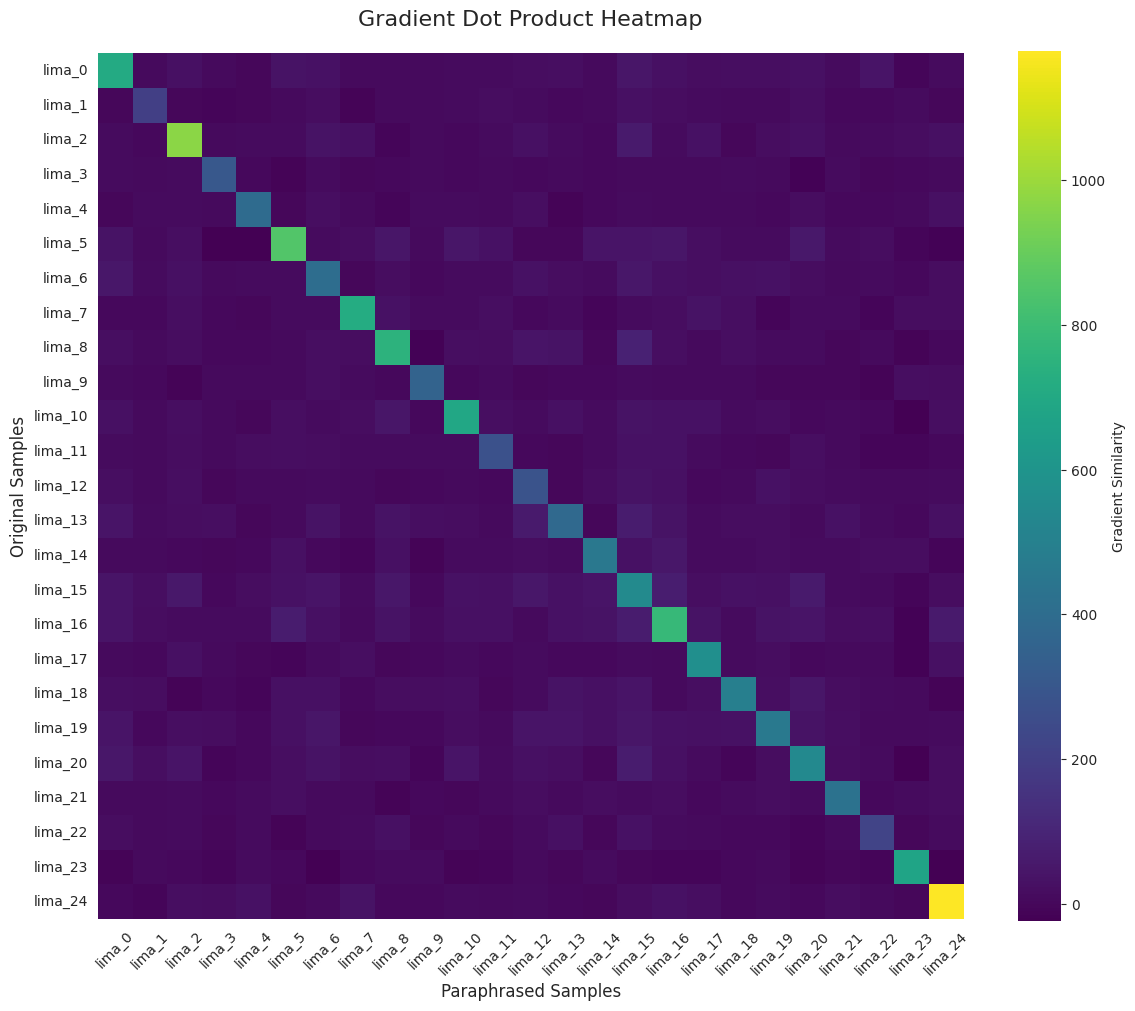
\includegraphics[width=1\textwidth]{figures/preliminary_analysis_dot_products.png}
    \caption{Preliminary analysis of gradient dot products between paraphrased and original samples.}
    \label{fig:preliminary_analysis_dot_products}
\end{figure}

\section{Dataset Examples}

\subsection{Paraphrased}\label{subsec:appendix_paraphrased_sample}
The paraphrased equivalent for the presented example for the \emph{LIMA} dataset illustrated in Subsection~\ref{subsec:lima_dataset}.
\\\\
Paraphrased user message $s_{p_{0_P}}$:
\begin{verbatim}
    Are brain cells capable of moving? Specifically, I'm referring to 
    long-distance migration, ideally occurring within the brain.
\end{verbatim}
Paraphrased assistant message $s_{p_{0_G}}$:
\begin{verbatim}
    The inquiry is quite extensive, and it’s important to recognize that the
    brain is made up not only of neurons but also of glial cells (supporting 
    cells) and pre-mitotic neuronal stem cells. Additionally, as critical 
    colleagues in research have pointed out, the developmental stage is 
    crucial, since the developing embryonic brain is significantly different 
    from the fully developed adult brain. Nonetheless, after reviewing various 
    studies, the answer to the question turns out to be surprisingly 
    straightforward: Yes, brain cells do migrate. In the adult brain, glial 
    cells are known to migrate (Klämbt, 2009). These glial cells perform 
    numerous functions, with a prominent example being oligodendrocytes, 
    which migrate over considerable distances to locate their target axons 
    and encase them to create the insulating myelin sheath 
    (Tsai and Miller, 2002). Neuronal stem cells also migrate long distances
    in response to injury (Imitola et al., 2004), moving from specific 
    stem-cell areas (such as the hippocampus and subventricular zone) to 
    other parts of the brain (Clarke, 2003). It has been demonstrated that 
    post-mitotic but non-differentiated neurons can migrate within the 
    adult brain in fish (Scott et al., 2012) and also in mammals and 
    non-human primates (Sawada et al., 2011). Unsurprisingly, glial cells, 
    stem cells, and neurons also undergo migration during embryonic 
    development. Most notably, post-mitotic neurons that are intended for 
    peripheral roles must migrate over relatively long distances from the 
    neural crest to their designated target areas 
    (Neuroscience, 2nd ed, Neuronal Migration).
\end{verbatim}

\subsection{Model-Generated}\label{subsec:appendix_model_generated_sample}
The model-generated equivalent for the presented example for the \emph{LIMA} dataset illustrated in Subsection~\ref{subsec:lima_dataset}.
\\\\
Model-generated user message $s_{m_{0_P}}$:
\begin{verbatim}
    Are brain cells capable of moving? Specifically, I'm referring to
    long-distance migration, ideally occurring within the brain.
\end{verbatim}
Model-generated assistant message $s_{m_{0_G}}$:
\begin{verbatim}
    Brain cells, such as neurons, are indeed capable of moving. This 
    movement is crucial for various functions, including communication 
    between neurons and the formation of neural networks. However, the 
    extent of brain cell movement is limited by the physical constraints
    of the brain's structure.

    Neurons are highly organized and interconnected, forming complex 
    networks that enable the brain to process and interpret information.
    The movement of neurons within these networks is facilitated by the 
    cytoskeleton, which provides structural support and allows for the 
    movement of the cell body.
    
    While brain cells can move within the brain, the movement is typically
    limited to short distances and is not as extensive as the movement of 
    neurons in other parts of the body. The brain's structure and the 
    limitations of its physical constraints prevent the movement of brain
    cells over long distances.
    ####
    Yes, brain cells can move, but it is limited to short distances within 
    the brain.
\end{verbatim}

\section{Results}

\subsection{Accuracy per Layer Component}

\subsubsection{Paraphrased}
\begin{figure}[ht]
    \centering
    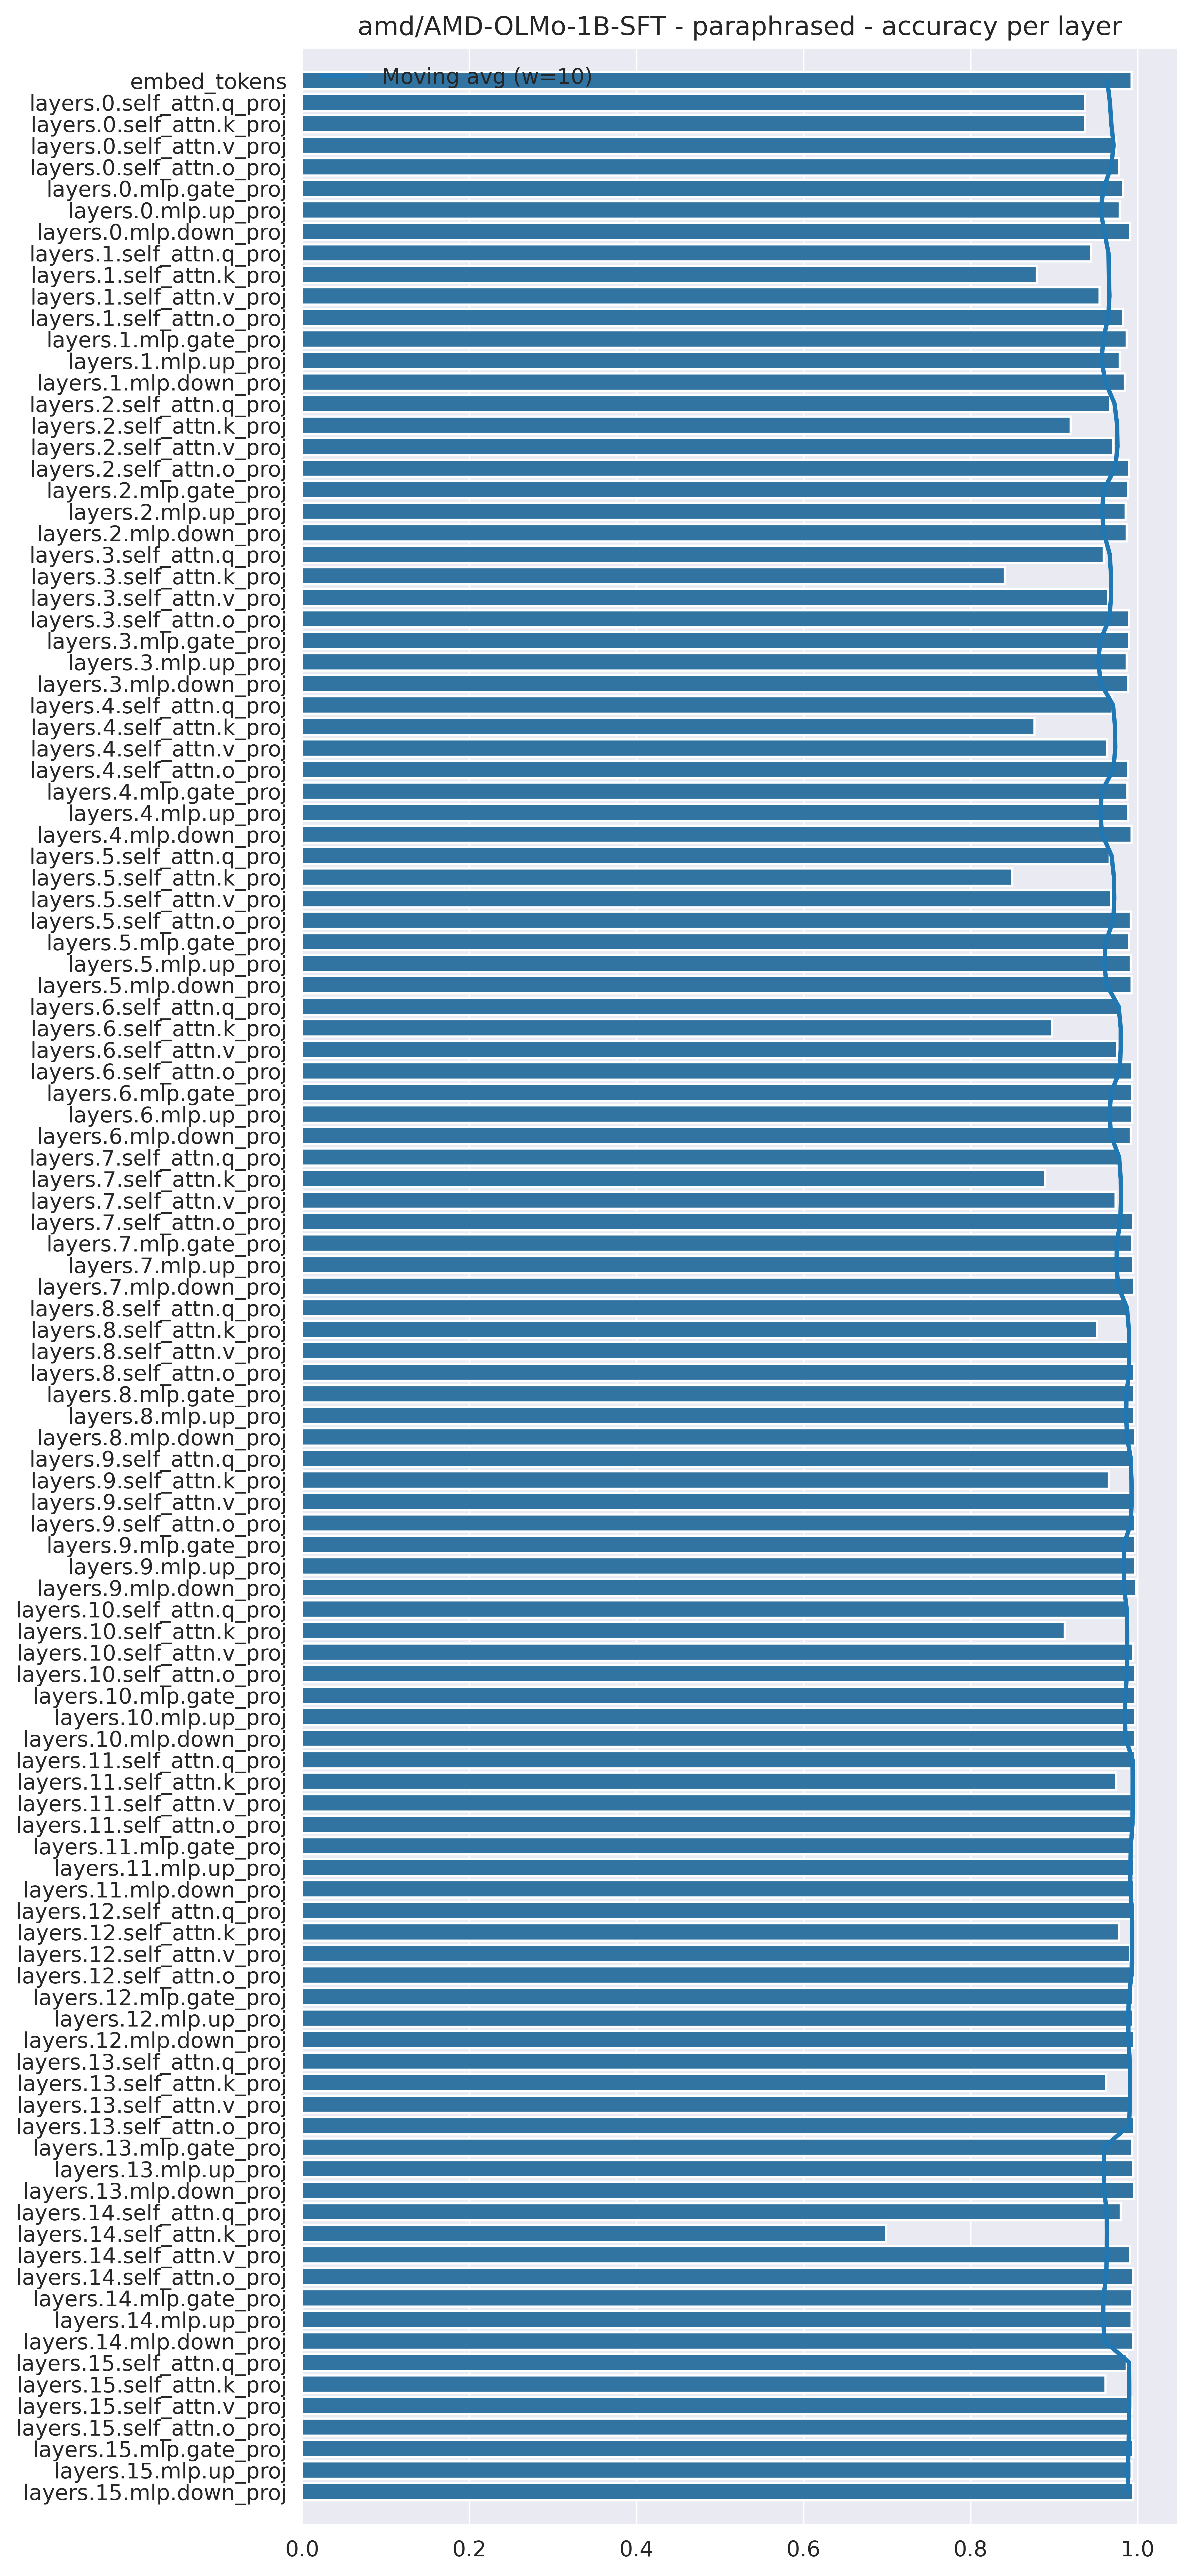
\includegraphics[width=0.63\textwidth]{figures/results/paraphrased/accuracy_per_layer.png}
    \caption{Accuracy per layer in the paraphrased setting}
    \label{fig:paraphrased_accuracy_per_layer}
\end{figure}

\subsubsection{Model-generated}
\begin{figure}[ht]
    \centering
    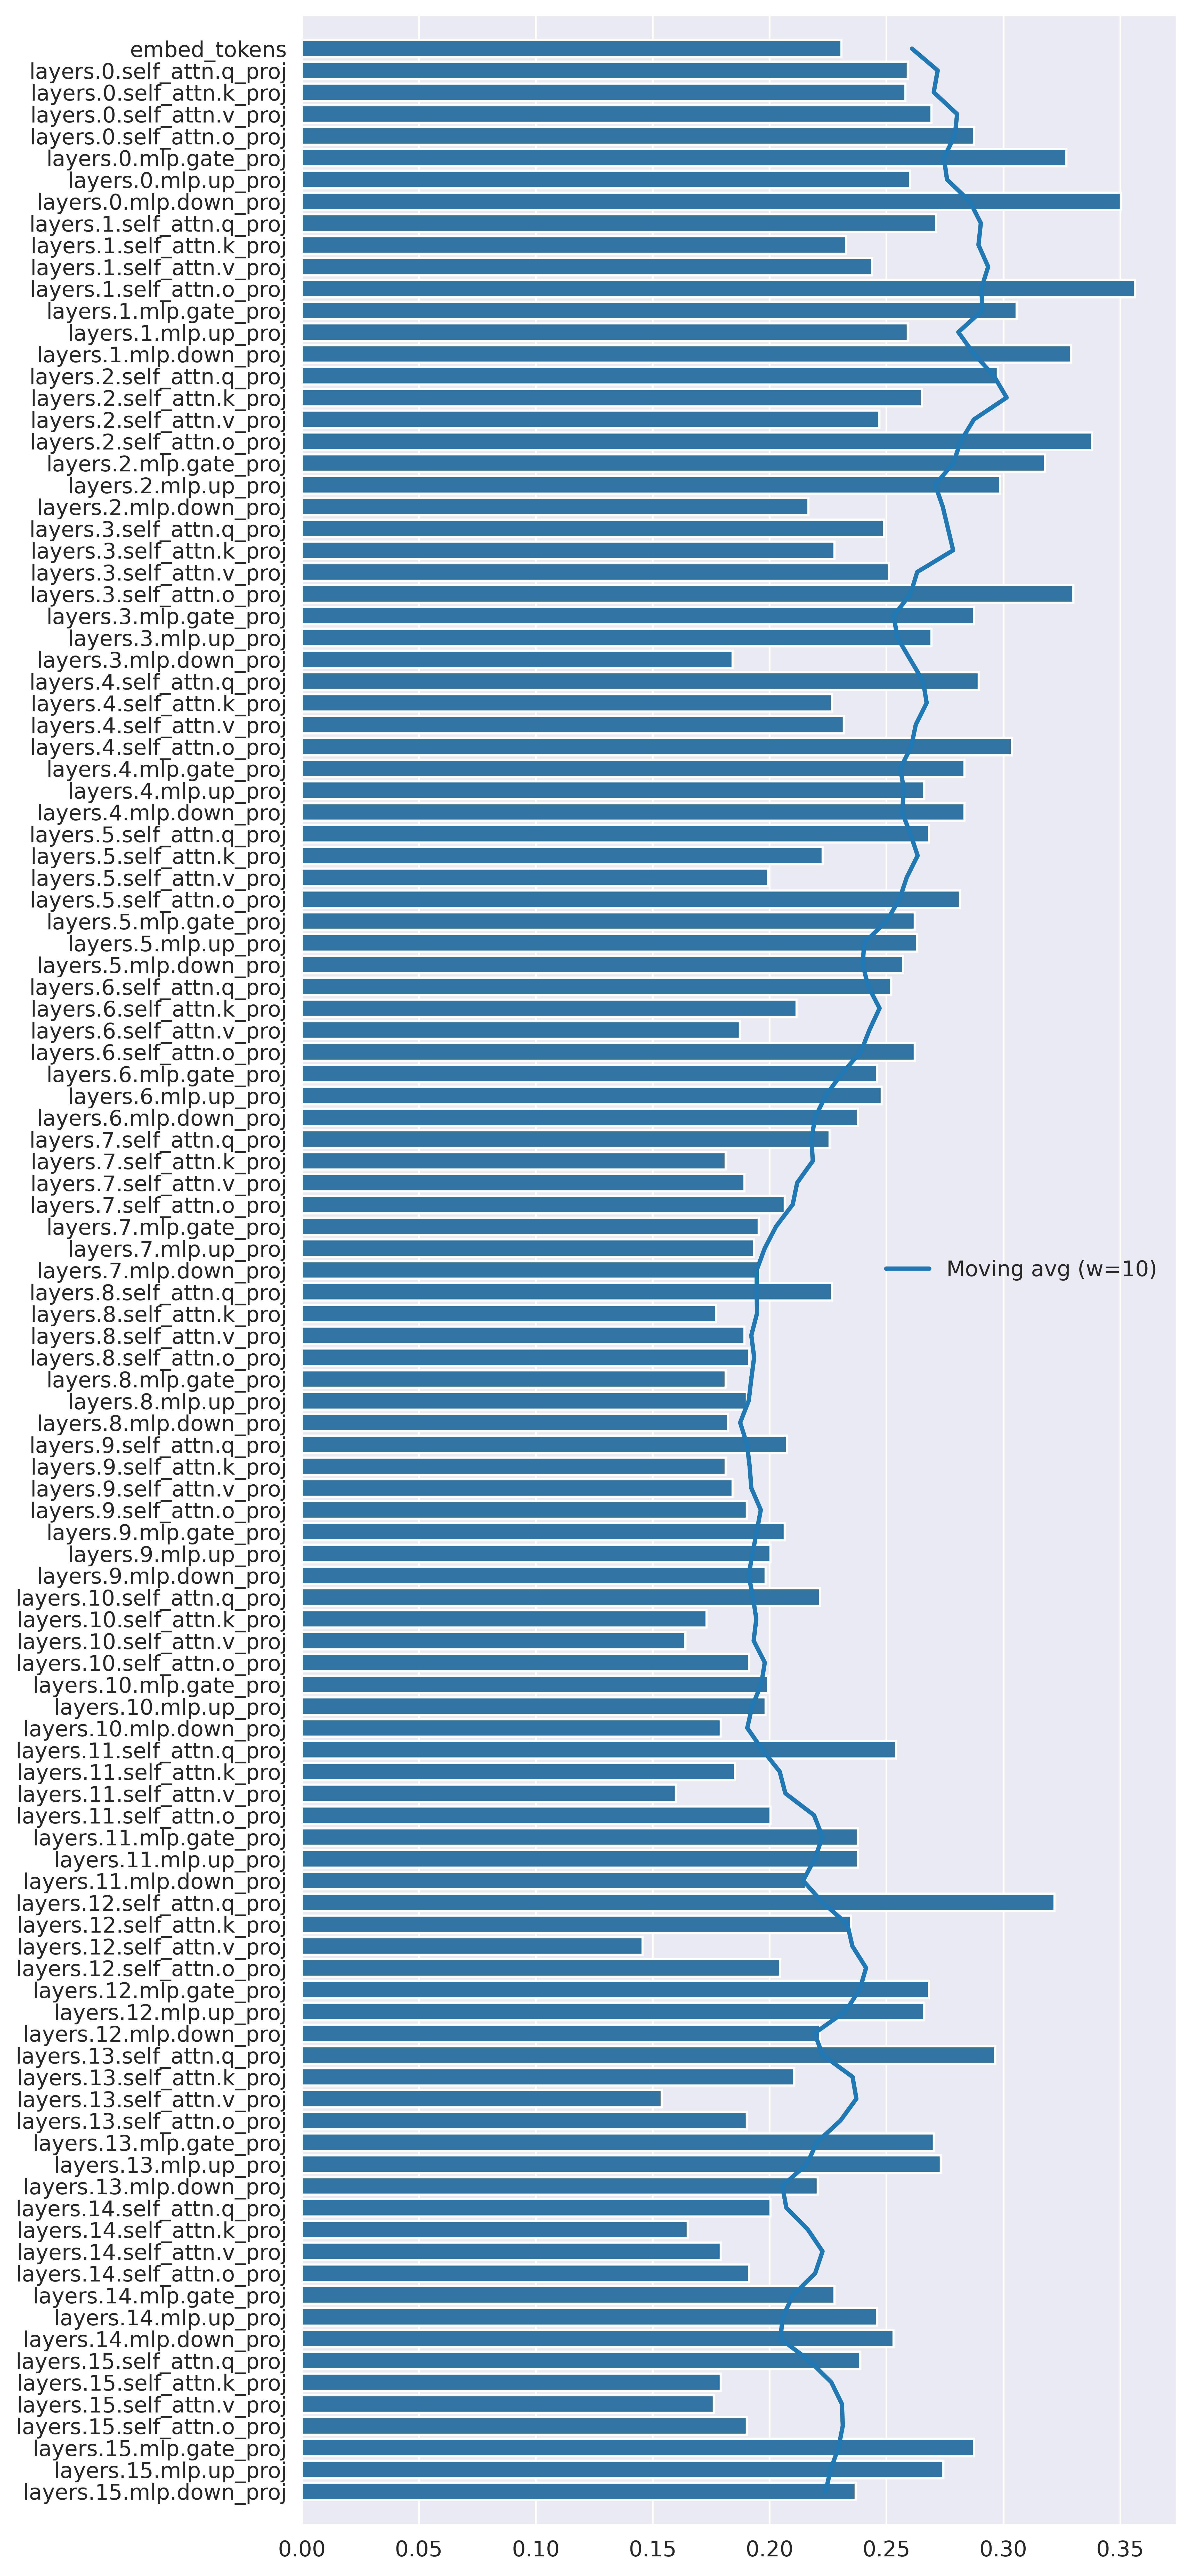
\includegraphics[width=0.63\textwidth]{figures/results/model-generated/accuracy_per_layer.png}
    \caption{Accuracy per layer in the model-generated setting}
    \label{fig:model_generated_accuracy_per_layer}
\end{figure}

\subsection{Comparison between Layer Components and Full Gradient}

\subsubsection{Paraphrased}
\begin{figure}[ht]
    \centering
    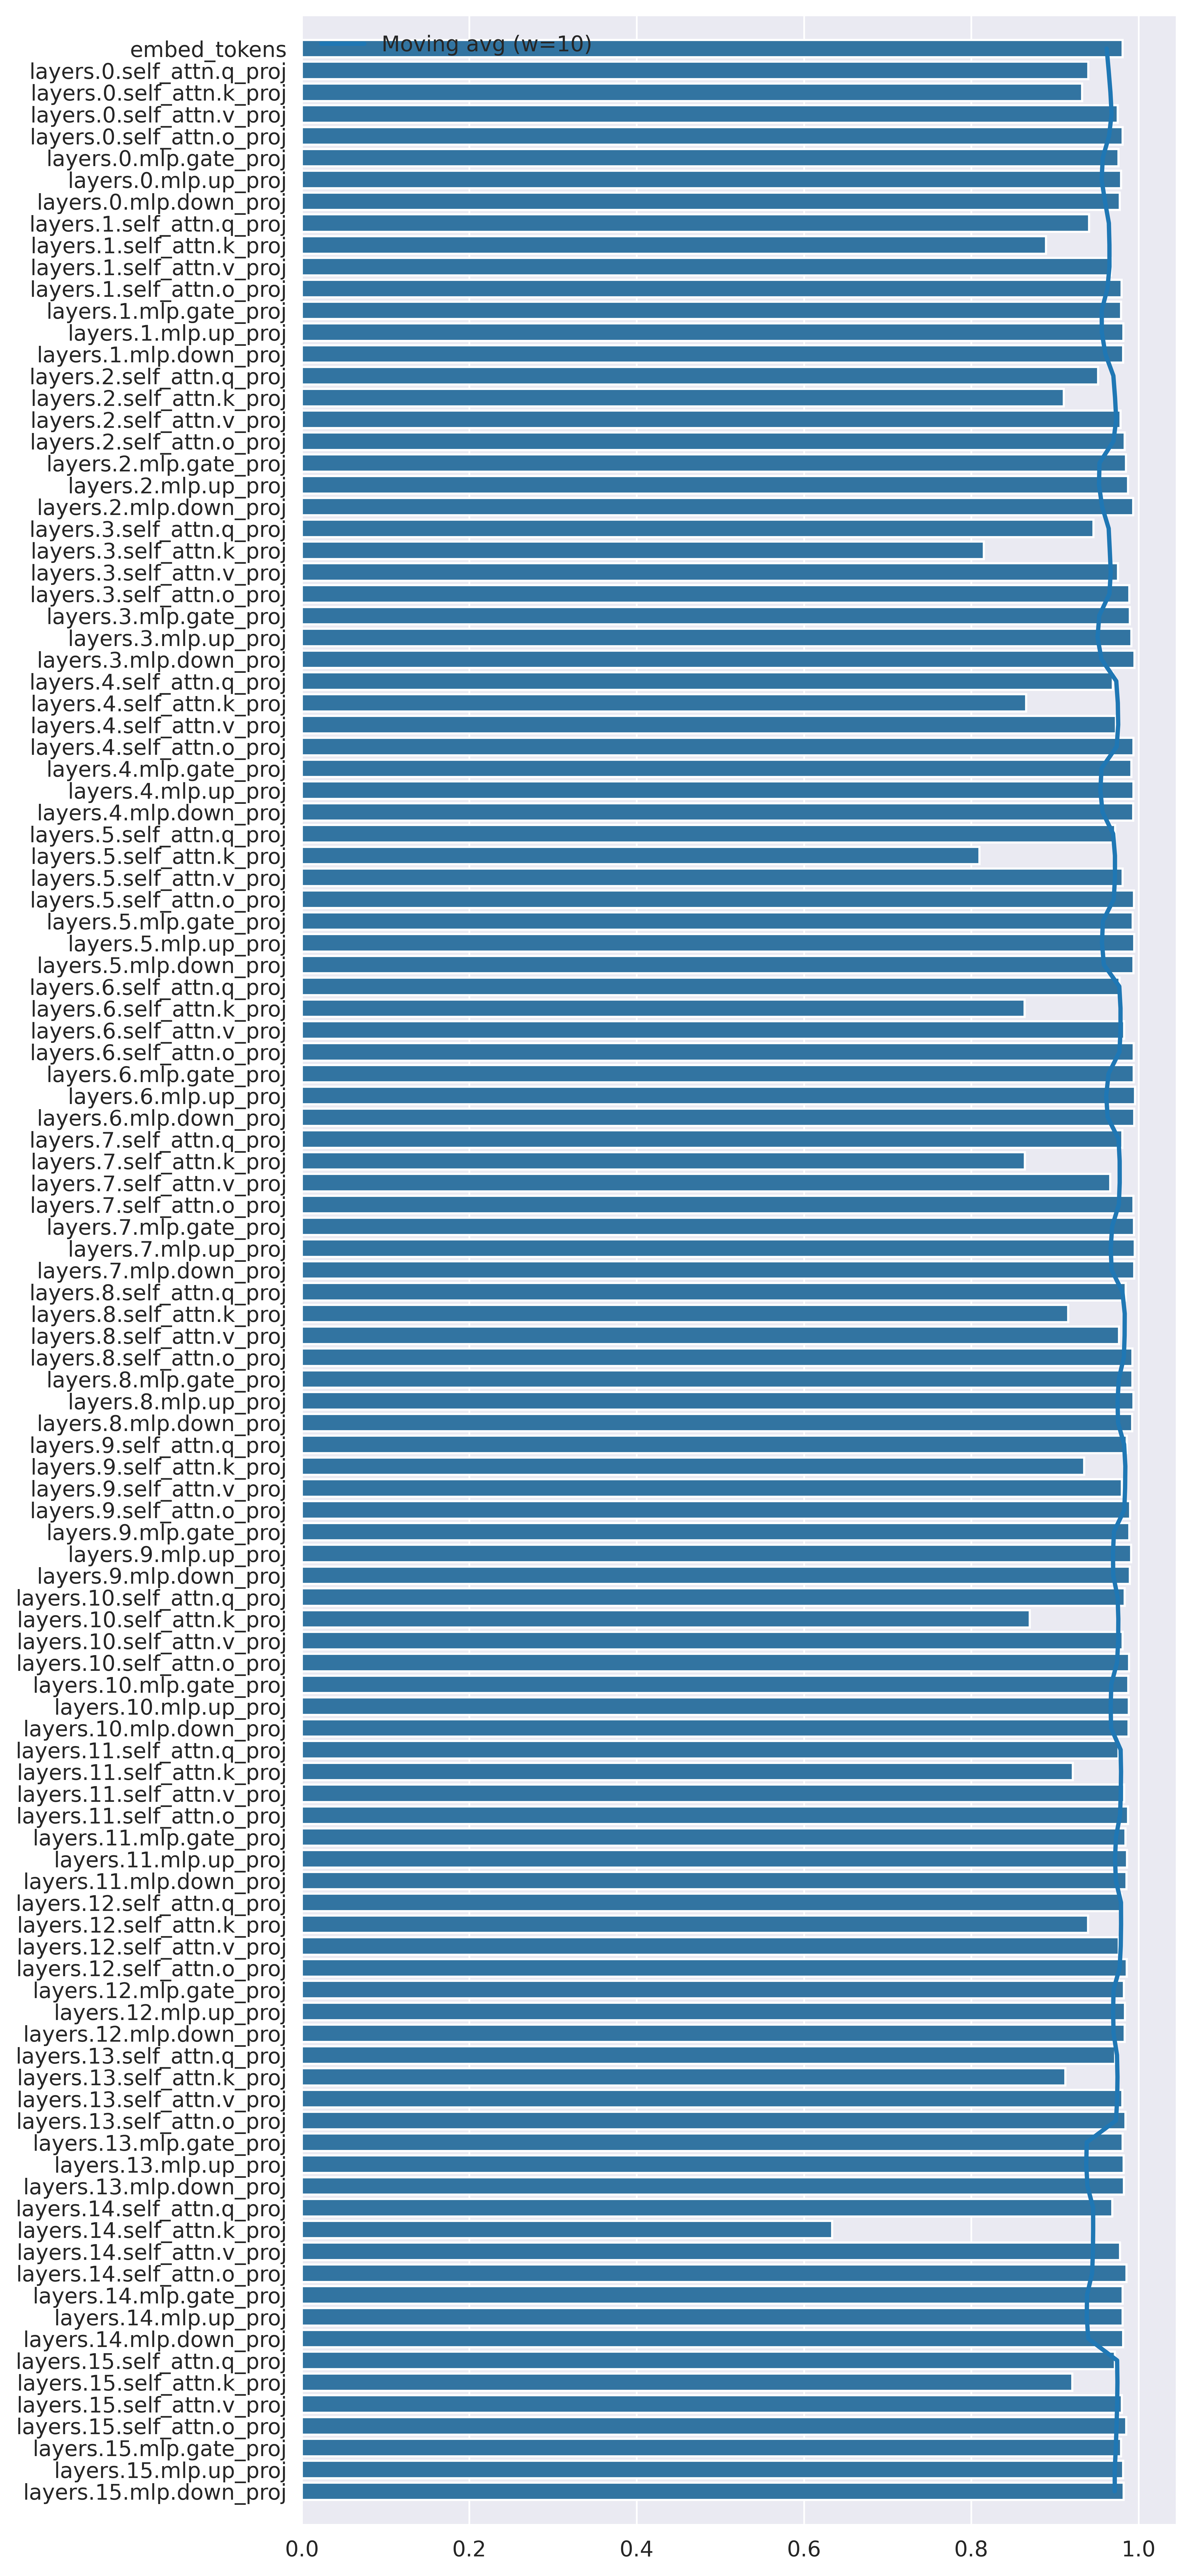
\includegraphics[width=0.63\textwidth]{figures/results/paraphrased/layer_comparison_full_gradient.png}
    \caption{Comparison of single layer component and full model gradient scores for the paraphrased setting.}
    \label{fig:paraphrased_layer_comparison_full_gradient}
\end{figure}

\subsubsection{Model-generated}

\subsubsection{Paraphrased}
\begin{figure}[ht]
    \centering
    \includegraphics[width=0.63\textwidth]{figures/results/model-generated/layer_comparison_full_gradient.png}
    \caption{Comparison of single layer component and full model gradient scores for the model-generated setting.}
    \label{fig:model_generated_layer_comparison_full_gradient}
\end{figure}

\section{Code and Repository}
The complete project code can be found on the following GitHub repository: \url{https://github.com/lukas-hinterleitner/master-thesis}.

	
\end{document}